\documentclass[a4paper,11pt,UKenglish,twoside,openright]{report}\usepackage[]{graphicx}\usepackage[]{color}
% maxwidth is the original width if it is less than linewidth
% otherwise use linewidth (to make sure the graphics do not exceed the margin)
\makeatletter
\def\maxwidth{ %
  \ifdim\Gin@nat@width>\linewidth
    \linewidth
  \else
    \Gin@nat@width
  \fi
}
\makeatother

\usepackage{Sweavel}



\usepackage{uiothesis}

\title{Identifying School Climate Variables Associated with Students' Financial Literacy Outcomes}
\subtitle{A Cross-Country Comparison\\Using {PISA} 2018 Data}
\author{Tony C. A. Tan}

\begin{document}

% Input faculty etc info
\duoforside[
    fac={Faculty of Educational Sciences},
    dept={Centre for Educational Measurement},
    program={Assessment, Measurement and Evaluation},
    date={Spring 2021},
%  printer={X-press printing house},
    short
]

% Change page numbering to roman
\pagenumbering{roman}

% Create an acknowledgement page
\thispagestyle{empty}

% This is where I generated the Chinese characters
%//ref http://www.akuziti.com/mb/
% I used font 24.Huawen Xingkai and 100 pixel
\vspace*{\fill}
\begin{figure*}[h]
    
\includegraphics[width=\textwidth]{./Figures/To-parents.png}
\end{figure*}
\begin{flushright}
To my parents
\end{flushright}
\vspace*{\fill}
%\newpage
\clearpage
\thispagestyle{empty}

\vspace*{3cm}

\begin{quote}
    \calligra\huge      % Changes the font to caligraphy and huge size.
\hyphenchar\font=-1     % Stops LaTeX from splitting/hyphenating words
Study hard what interests you the most in the most undisciplined, irreverent and original manner possible.
\end{quote}

\begin{figure*}[h]
    \flushright
    
\includegraphics[width=0.50\textwidth]{./Figures/Feynman-Signature.jpg}
\end{figure*}
\vspace*{-1cm}

%\begin{flushright}
%--- Richard P. Feynman
%\end{flushright}

% Set 1.5-spacing or 2-spacing from here on.
\onehalfspacing
%\doublespacing

\setcounter{page}{0}
% End of acknowledgement page

% Put Table of Content here
\tableofcontents

% Put a List of Tables here
\cleardoublepage
\listoftables

% Put a List of Figures here
\cleardoublepage
\listoffigures

% Change page numbering back to arabic
\cleardoublepage
\pagenumbering{arabic}




% Acknowledgement
%<<child="Chapters/Acknowledgement.Rnw", tidy=FALSE, message=FALSE, warning=FALSE>>=
%@

% Popular Abstract
%<<child="Chapters/Abstract0.Rnw", tidy=FALSE, message=FALSE, warning=FALSE>>=
%@

% Abstract
%<<child="Chapters/Abstract1.Rnw", tidy=FALSE, message=FALSE, warning=FALSE>>=
%@

% Chapter 1 Introduction

\chapter{Introduction}
\label{chp:1}

%\epigraph{If you think education is expensive, try ignorance}{Derek Bok}

This is a line that recently got added.

\section{Broad motivations}

As shown in \cref{fig:1.1}, the world is not that bad.

\section{Quick definitions of key terms}

\subsection{Financial literacy vs finance}

\subsection{Flow vs stock: teaching vs assessment of financial literacy}

\section{My topic(s)}

\section{Zooming out: Why this topic is important?}


\parencite{abubakar:2020,agarwal:2015,agnew:2015a,agnew:2015b,agyei:2018,akbenselcuk:2014,ali:2014,allgood:2016,amagir:2018,aprea:2015,arceogomez:2017,arellano:2014,arellano:2018,arthur:2012,atkinson:2011,bartholomae:2016,batsaikhan:2018,becchetti:2013,beckmann:2020,behrman:2012,bel:2015,belas:2016,bernheim:2001,birbili:2015,blue:2014a,blue:2014b,blue:2017,blue:2018,blue:2020,boisclair:2017,bongini:2012,bottazzi:2016,bover:2018,bover:2020,bowen:2002,bray:1995,breitbach:2016,brimble:2013,brown:2013,brown:2016,brown:2018,bucciol:2020,bucherkoenen:2016,caliendo:2013,cameron:2013,campioni:2017,carlin:2012a,carlin:2012b,carvalho:2020,chambers:2018,chambers:2019,chatfield:1978,chen:2018,chiang:2020,ciemleja:2014a,ciemleja:2014b,cole:2009,cole:2016,collins:2013,connolly:2015,cordero:2019,cude:2016,cupak;2018b,cupak:2018a,cupak:2018c,curugan:2020,danes:2007,davies:2016,davoli:2020,debeckker:2019,debeckker:2020,driva:2016,eickelmann:2016,emmons:2005,eniola:2016,erner:2016,ethics,fabris:2016,farinella:2017,fernandes:2014,ferrari:2019,FLdata,fonseca:2012,fornero:2019,forster:2017,fraczek:2015,frisancho:2019,garder:1985,garg:2018,geiger:2016,gomes:2020,goyal:2020,gramatki:2017,grohmann:2015,grohmann:2016,grohmann:2018,gudmunson:2011,gudmunson:2016,guest:2018,hanushek:2012a,hanushek:2012b,happ:2016,hastings:2013,hdr:data,henderson:2020,hira:2016,ho:2020,holtsch:2016,huston:2010,huston:2012,ibarra:2019,intsvy,janssen:2019,jappelli:2010,jappelli:2013,jappelli:2015,jorgensen:2010,jüttler:2016,kaiser:2020,kalmi:2018,karakurumozdemir:2019,kell:2014,kenayathulla:2020,khalil:2020,khan:2017,khoirunnisaa:2020,kiliyanni:2016,kim:2020,klapper:2019,klieme:2020,kosor:2020,kunovskaya:2014,laukaityte:2018,leumann:2016,li:2020,liaqat:2020,longobardi:2017,longobardi:2018,loprete:2013,lusardi:2007,lusardi:2008,lusardi:2010,lusardi:2011,lusardi:2012,lusardi:2013,lusardi:2014,lusardi:2015a,lusardi:2015b,lusardi:2016,lusardi:2017,lusardi:2019a,lusardi:2019b,mancebon:2015,mancebon:2019,mandell:2009,mandmaa:2020,marsh:2004,marsh:2012,marsh:2019,matheson:2020,mitchell:2015,mohammadpour:2013,morenoherrero:2018a,morenoherrero:2018b,mountain:2020,norvilitis:2006,norvilitis:2010,nurhasanah:2020,oberrauch:2019,oecd:2005,oecd:2009,olivermarquez:2020,opletalova:2015,page:2020,paolostella:2020,pesando:2018,peugh:2010,pinto:2011,pinto:2012,pinto:2013,pokropek:2016,potrich:2015,potrich:2016,preston:2019,R,remund:2010,riitsalu:2016,rinaldi:2012,rodriguez:2020,rohatgi:2020,rubin:1987,rust:2014,rustomfram:2015,rutkowski:2010,savard:2020,sawatzki:2020,schmeiser:2013,schuhen:2014,schurkmann:2013,sellar:2013,serido:2016,shadish:2002,shen:2016,shim:2009,shim:2010,siegfried:2016,silgoner:2015,skagerlund:2018,soderlund:2020,sole:2014,spataro:2017,stanisavjevic:2018,stolper:2017,strahija:2020,strietholt:2018,sun:2012,sutter:2020,taylor:2013,tchatoka:2020,teenharari:2016,tezel:2015,thomas:2018,thomson:2017,titko:2015a,titko:2015b,toosi:2020,vale:2020,vancampenhout:2015,vanrooij:2011,vondavier:2014,vyvyan:2014,wang:2015,wang:2020,wastad:2016,willis:2008,worldbank:data,young:2013,young:2015,youshino:2015,zhu:2012,zhu:2015,zokaityte:2016,utkarsh:2020,grund:2020,guttman:1944,goodman:1975,green:1956,ozkale:2020,endsley:2020}

% Chapter 2 Theoretical framework

\chapter{Conceptual Framework}
\label{chp:2}

\section{In-depth definitions of ``financial literacy''}

\subsection{Every term my readers need in order to understand my research question}

\subsection{Survey not only PISA but also alternative definitions, even critiques of such definitions}

\subsection{Any practices that are common in maths/literature but uncommon in financial literacy? Meaning? Implies?}

\newpage

\section{Country-level Financial Knowledge Index}

PISA 2018 financial literacy dataset \parencite{FLdata} provides rich information about students and schools. For the purpose of cross-country comparison, however, the country-level financial literacy information must be addressed separately by the researchers. Earlier attempts such as \textcite{morenoherrero:2018a} approximated this information using a variable ``quality of math and science education'' to control for country-level differences since consensus is yet to emerge about the most appropriate measure for countries' financial knowledge. Inspired by the UN's approach to forming Human Development Indices, a recent publication by \textcite{olivermarquez:2020} proposed a macroeconomic measure for countries' general financial knowledge levels by examining their economic capability, educational training, existing practices in the financial markets as well as incentives to interact with financial products. More specifically, the authors considered a country's economic capability, represented by its GDP per capita, to be a key dimension in bringing about its financial knowledge index (FKI). Secondly, literature converges on the importance of educational training for a country's financial knowledge capability \parencite{oecd:2005}. Thirdly, countries with regular engagement with sophisticated financial products and financial markets should possess higher FKI. Lastly, countries with higher aggregate consumption levels and with ageing populations are likely to possess higher FKI due to more frequent exposure and pressure in retirement provision, respetively. Macroeconomic data needed for these computations can be sourced from the World Bank \parencite{worldbank:data} and the United Nations' \textit{Human Development Reports} \parencite{hdr:data}.

Combining individual and institutional data cources can be a productive approach in international large-scale assessment (ILSA) research. According to the framework for comparative education analyses \parencite{bray:1995}, this project extends education outcome measures to a country level, addresses the aspect of society and labour market, and relates countries' entire populations to ILSA research \parencite{strietholt:2018}. By combining education outcome data with countries' economic performance indicators, this project remains most comparable to \textcite{hanushek:2012a}---while these authors looked into the relationship between countries' education achievement and their GDP growth, the current investigation highlights how countries' GDP, along with other macroeconomic practices, in turn systematically impacts on their youth's educational performance.

\newpage

% Table generated by Excel2LaTeX from sheet 'Sheet2'
\ltable{tab:Missing}{Percentages of Missing Values}{
      \begin{tabular}{ccrrrrrrrrrrrrrrrrrrrr}
      \toprule
      CNT   &       & \multicolumn{1}{c}{\rotatebox{90}{\texttt{MALE}}} & \multicolumn{1}{c}{\rotatebox{90}{\texttt{IMMI1GEN}}} & \multicolumn{1}{c}{\rotatebox{90}{\texttt{IMMI2GEN}}} & \multicolumn{1}{c}{\rotatebox{90}{\texttt{ESCS}}} & \multicolumn{1}{c}{\rotatebox{90}{\texttt{FCFMLRTY}}} & \multicolumn{1}{c}{\rotatebox{90}{\texttt{FLCONFIN}}} & \multicolumn{1}{c}{\rotatebox{90}{\texttt{PERFEED}}} & \multicolumn{1}{c}{\rotatebox{90}{\texttt{TEACHINT}}} & \multicolumn{1}{c}{\rotatebox{90}{\texttt{FLSCHOOL}}} & \multicolumn{1}{c}{\rotatebox{90}{\texttt{DISCRIM}$^\dagger$}} & \multicolumn{1}{c}{\rotatebox{90}{\texttt{BELONG}}} & \multicolumn{1}{c}{\rotatebox{90}{\texttt{BULLY}}} & \multicolumn{1}{c}{\rotatebox{90}{\texttt{FLFAMILY}}} & \multicolumn{1}{c}{\rotatebox{90}{\texttt{CURSUPP}$^\dagger$}} & \multicolumn{1}{c}{\rotatebox{90}{\texttt{PASCHPOL}$^\dagger$}} & \multicolumn{1}{c}{\rotatebox{90}{\texttt{W\_SCH}}} & \multicolumn{1}{c}{\rotatebox{90}{\texttt{PRIVATE}}} & \multicolumn{1}{c}{\rotatebox{90}{\texttt{STRATIO}}} & \multicolumn{1}{c}{\rotatebox{90}{\texttt{EDUST}}} & \multicolumn{1}{c}{\rotatebox{90}{\texttt{STAFFST}}} \\
      \midrule
      BGR$^\dagger$   &       & 0     & \cellcolor[rgb]{ 1,  .945,  .945}6 & \cellcolor[rgb]{ 1,  .945,  .945}6 & \cellcolor[rgb]{ 1,  .973,  .973}3 & \cellcolor[rgb]{ 1,  .882,  .882}12 & \cellcolor[rgb]{ 1,  .733,  .733}27 & \cellcolor[rgb]{ 1,  .898,  .898}10 & \cellcolor[rgb]{ 1,  .906,  .906}10 & \cellcolor[rgb]{ 1,  .792,  .792}21 & \cellcolor[rgb]{ 1,  .722,  .722}28 & \cellcolor[rgb]{ 1,  .808,  .808}19 & \cellcolor[rgb]{ 1,  .694,  .694}31 & \cellcolor[rgb]{ 1,  .784,  .784}22 & \cellcolor[rgb]{ 1,  0,  0}100 & \cellcolor[rgb]{ 1,  0,  0}100 & 0     & \cellcolor[rgb]{ 1,  0,  0}100 & \cellcolor[rgb]{ 1,  .922,  .922}8 & \cellcolor[rgb]{ 1,  .973,  .973}3 & \cellcolor[rgb]{ 1,  .973,  .973}3 \\
      BRA   &       & 0     & \cellcolor[rgb]{ 1,  .949,  .949}5 & \cellcolor[rgb]{ 1,  .949,  .949}5 & \cellcolor[rgb]{ 1,  .98,  .98}2 & \cellcolor[rgb]{ 1,  .878,  .878}12 & \cellcolor[rgb]{ 1,  .667,  .667}34 & \cellcolor[rgb]{ 1,  .91,  .91}9 & \cellcolor[rgb]{ 1,  .925,  .925}8 & \cellcolor[rgb]{ 1,  .796,  .796}21 & \cellcolor[rgb]{ 1,  .643,  .643}36 & \cellcolor[rgb]{ 1,  .776,  .776}23 & \cellcolor[rgb]{ 1,  .6,  .6}40 & \cellcolor[rgb]{ 1,  .765,  .765}24 & \cellcolor[rgb]{ 1,  .831,  .831}17 & \cellcolor[rgb]{ 1,  .816,  .816}19 & 0     & 0     & \cellcolor[rgb]{ 1,  .882,  .882}12 & \cellcolor[rgb]{ 1,  .941,  .941}6 & \cellcolor[rgb]{ 1,  .933,  .933}7 \\
      CAN$^\dagger$   &       & 0     & \cellcolor[rgb]{ 1,  .933,  .933}7 & \cellcolor[rgb]{ 1,  .933,  .933}7 & \cellcolor[rgb]{ 1,  .953,  .953}5 & \cellcolor[rgb]{ 1,  .894,  .894}11 & \cellcolor[rgb]{ 1,  .851,  .851}15 & \cellcolor[rgb]{ 1,  0,  0}100 & \cellcolor[rgb]{ 1,  0,  0}100 & \cellcolor[rgb]{ 1,  .875,  .875}13 & \cellcolor[rgb]{ 1,  0,  0}100 & \cellcolor[rgb]{ 1,  .925,  .925}8 & \cellcolor[rgb]{ 1,  .859,  .859}14 & \cellcolor[rgb]{ 1,  .867,  .867}14 & \cellcolor[rgb]{ 1,  0,  0}100 & \cellcolor[rgb]{ 1,  0,  0}100 & 0     & 0     & \cellcolor[rgb]{ 1,  0,  0}100 & \cellcolor[rgb]{ 1,  .988,  .988}2 & \cellcolor[rgb]{ 1,  .984,  .984}2 \\
      CHL   &       & 0     & \cellcolor[rgb]{ 1,  .961,  .961}4 & \cellcolor[rgb]{ 1,  .961,  .961}4 & \cellcolor[rgb]{ 1,  .976,  .976}3 & \cellcolor[rgb]{ 1,  .906,  .906}10 & \cellcolor[rgb]{ 1,  .769,  .769}24 & \cellcolor[rgb]{ 1,  .953,  .953}5 & \cellcolor[rgb]{ 1,  .961,  .961}4 & \cellcolor[rgb]{ 1,  .875,  .875}13 & \cellcolor[rgb]{ 1,  .706,  .706}30 & \cellcolor[rgb]{ 1,  .851,  .851}15 & \cellcolor[rgb]{ 1,  .663,  .663}34 & \cellcolor[rgb]{ 1,  .855,  .855}15 & \cellcolor[rgb]{ 1,  .918,  .918}9 & \cellcolor[rgb]{ 1,  .918,  .918}8 & 0     & 0     & \cellcolor[rgb]{ 1,  .82,  .82}18 & \cellcolor[rgb]{ 1,  .906,  .906}9 & \cellcolor[rgb]{ 1,  .914,  .914}9 \\
      ESP   &       & 0     & \cellcolor[rgb]{ 1,  .973,  .973}3 & \cellcolor[rgb]{ 1,  .973,  .973}3 & \cellcolor[rgb]{ 1,  .984,  .984}2 & \cellcolor[rgb]{ 1,  .957,  .957}5 & \cellcolor[rgb]{ 1,  .792,  .792}21 & \cellcolor[rgb]{ 1,  .973,  .973}3 & \cellcolor[rgb]{ 1,  .98,  .98}2 & \cellcolor[rgb]{ 1,  .929,  .929}7 & \cellcolor[rgb]{ 1,  .757,  .757}25 & \cellcolor[rgb]{ 1,  .91,  .91}9 & \cellcolor[rgb]{ 1,  .718,  .718}29 & \cellcolor[rgb]{ 1,  .918,  .918}8 & \cellcolor[rgb]{ 1,  0,  0}100 & \cellcolor[rgb]{ 1,  0,  0}100 & 0     & 0     & \cellcolor[rgb]{ 1,  .89,  .89}11 & \cellcolor[rgb]{ 1,  .949,  .949}5 & \cellcolor[rgb]{ 1,  .945,  .945}6 \\
      EST   &       & 0     & \cellcolor[rgb]{ 1,  .969,  .969}3 & \cellcolor[rgb]{ 1,  .969,  .969}3 & \cellcolor[rgb]{ 1,  .976,  .976}3 & \cellcolor[rgb]{ 1,  .957,  .957}4 & \cellcolor[rgb]{ 1,  .925,  .925}8 & \cellcolor[rgb]{ 1,  .969,  .969}3 & \cellcolor[rgb]{ 1,  .973,  .973}3 & \cellcolor[rgb]{ 1,  .945,  .945}6 & \cellcolor[rgb]{ 1,  .914,  .914}9 & \cellcolor[rgb]{ 1,  .957,  .957}5 & \cellcolor[rgb]{ 1,  .898,  .898}11 & \cellcolor[rgb]{ 1,  .941,  .941}6 & \cellcolor[rgb]{ 1,  0,  0}100 & \cellcolor[rgb]{ 1,  0,  0}100 & 0     & 0     & 0     & 0     & 0 \\
      FIN$^\dagger$   &       & 0     & \cellcolor[rgb]{ 1,  .98,  .98}2 & \cellcolor[rgb]{ 1,  .98,  .98}2 & \cellcolor[rgb]{ 1,  .984,  .984}2 & \cellcolor[rgb]{ 1,  .957,  .957}4 & \cellcolor[rgb]{ 1,  .898,  .898}10 & \cellcolor[rgb]{ 1,  .973,  .973}3 & \cellcolor[rgb]{ 1,  .973,  .973}3 & \cellcolor[rgb]{ 1,  .937,  .937}6 & \cellcolor[rgb]{ 1,  0,  0}100 & \cellcolor[rgb]{ 1,  .937,  .937}6 & \cellcolor[rgb]{ 1,  .894,  .894}11 & \cellcolor[rgb]{ 1,  .933,  .933}7 & \cellcolor[rgb]{ 1,  0,  0}100 & \cellcolor[rgb]{ 1,  0,  0}100 & 0     & \cellcolor[rgb]{ 1,  0,  0}100 & \cellcolor[rgb]{ 1,  .98,  .98}2 & \cellcolor[rgb]{ 1,  .925,  .925}7 & \cellcolor[rgb]{ 1,  .925,  .925}7 \\
      GEO   &       & 0     & \cellcolor[rgb]{ 1,  .949,  .949}5 & \cellcolor[rgb]{ 1,  .949,  .949}5 & \cellcolor[rgb]{ 1,  .984,  .984}2 & \cellcolor[rgb]{ 1,  .914,  .914}9 & \cellcolor[rgb]{ 1,  .737,  .737}26 & \cellcolor[rgb]{ 1,  .906,  .906}9 & \cellcolor[rgb]{ 1,  .914,  .914}9 & \cellcolor[rgb]{ 1,  .827,  .827}17 & \cellcolor[rgb]{ 1,  0,  0}100 & \cellcolor[rgb]{ 1,  .855,  .855}15 & \cellcolor[rgb]{ 1,  .784,  .784}22 & \cellcolor[rgb]{ 1,  .796,  .796}21 & \cellcolor[rgb]{ 1,  .965,  .965}4 & \cellcolor[rgb]{ 1,  .953,  .953}5 & 0     & 0     & \cellcolor[rgb]{ 1,  .988,  .988}1 & \cellcolor[rgb]{ 1,  .984,  .984}2 & \cellcolor[rgb]{ 1,  .98,  .98}2 \\
      IDN   &       & 0     & \cellcolor[rgb]{ 1,  .976,  .976}3 & \cellcolor[rgb]{ 1,  .976,  .976}3 & \cellcolor[rgb]{ 1,  .996,  .996}1 & \cellcolor[rgb]{ 1,  .969,  .969}3 & \cellcolor[rgb]{ 1,  .945,  .945}6 & \cellcolor[rgb]{ 1,  .973,  .973}3 & \cellcolor[rgb]{ 1,  .98,  .98}2 & \cellcolor[rgb]{ 1,  .953,  .953}5 & \cellcolor[rgb]{ 1,  .969,  .969}3 & \cellcolor[rgb]{ 1,  .976,  .976}2 & \cellcolor[rgb]{ 1,  .949,  .949}5 & \cellcolor[rgb]{ 1,  .949,  .949}5 & \cellcolor[rgb]{ 1,  0,  0}100 & \cellcolor[rgb]{ 1,  0,  0}100 & 0     & 0     & \cellcolor[rgb]{ 1,  .773,  .773}23 & \cellcolor[rgb]{ 1,  .863,  .863}14 & \cellcolor[rgb]{ 1,  .863,  .863}14 \\
      ITA   &       & 0     & \cellcolor[rgb]{ 1,  .965,  .965}4 & \cellcolor[rgb]{ 1,  .965,  .965}4 & \cellcolor[rgb]{ 1,  .976,  .976}3 & \cellcolor[rgb]{ 1,  .933,  .933}7 & \cellcolor[rgb]{ 1,  .827,  .827}17 & \cellcolor[rgb]{ 1,  .957,  .957}4 & \cellcolor[rgb]{ 1,  .961,  .961}4 & \cellcolor[rgb]{ 1,  .902,  .902}10 & \cellcolor[rgb]{ 1,  .769,  .769}23 & \cellcolor[rgb]{ 1,  .902,  .902}10 & \cellcolor[rgb]{ 1,  .733,  .733}27 & \cellcolor[rgb]{ 1,  .882,  .882}12 & \cellcolor[rgb]{ 1,  .847,  .847}16 & \cellcolor[rgb]{ 1,  .835,  .835}17 & 0     & 0     & \cellcolor[rgb]{ 1,  .906,  .906}9 & \cellcolor[rgb]{ 1,  .969,  .969}3 & \cellcolor[rgb]{ 1,  .973,  .973}3 \\
      LTU   &       & 0     & \cellcolor[rgb]{ 1,  .976,  .976}3 & \cellcolor[rgb]{ 1,  .976,  .976}3 & \cellcolor[rgb]{ 1,  .973,  .973}3 & \cellcolor[rgb]{ 1,  .961,  .961}4 & \cellcolor[rgb]{ 1,  .882,  .882}12 & \cellcolor[rgb]{ 1,  .973,  .973}3 & \cellcolor[rgb]{ 1,  .976,  .976}3 & \cellcolor[rgb]{ 1,  .949,  .949}5 & \cellcolor[rgb]{ 1,  .831,  .831}17 & \cellcolor[rgb]{ 1,  .925,  .925}8 & \cellcolor[rgb]{ 1,  .8,  .8}20 & \cellcolor[rgb]{ 1,  .937,  .937}7 & \cellcolor[rgb]{ 1,  0,  0}100 & \cellcolor[rgb]{ 1,  0,  0}100 & 0     & 0     & 0     & 0     & 0 \\
      LVA$^\dagger$   &       & 0     & \cellcolor[rgb]{ 1,  .98,  .98}2 & \cellcolor[rgb]{ 1,  .98,  .98}2 & \cellcolor[rgb]{ 1,  .98,  .98}2 & \cellcolor[rgb]{ 1,  .949,  .949}5 & \cellcolor[rgb]{ 1,  .91,  .91}9 & \cellcolor[rgb]{ 1,  .973,  .973}3 & \cellcolor[rgb]{ 1,  .976,  .976}3 & \cellcolor[rgb]{ 1,  .937,  .937}6 & \cellcolor[rgb]{ 1,  .867,  .867}14 & \cellcolor[rgb]{ 1,  .937,  .937}6 & \cellcolor[rgb]{ 1,  .851,  .851}15 & \cellcolor[rgb]{ 1,  .933,  .933}7 & \cellcolor[rgb]{ 1,  0,  0}100 & \cellcolor[rgb]{ 1,  0,  0}100 & 0     & \cellcolor[rgb]{ 1,  0,  0}100 & \cellcolor[rgb]{ 1,  .937,  .937}6 & \cellcolor[rgb]{ 1,  .969,  .969}3 & \cellcolor[rgb]{ 1,  .965,  .965}4 \\
      NLD$^\dagger$   &       & 0     & \cellcolor[rgb]{ 1,  .973,  .973}3 & \cellcolor[rgb]{ 1,  .973,  .973}3 & \cellcolor[rgb]{ 1,  .98,  .98}2 & \cellcolor[rgb]{ 1,  .973,  .973}3 & \cellcolor[rgb]{ 1,  .953,  .953}5 & \cellcolor[rgb]{ 1,  .976,  .976}3 & \cellcolor[rgb]{ 1,  .976,  .976}2 & \cellcolor[rgb]{ 1,  .965,  .965}4 & \cellcolor[rgb]{ 1,  0,  0}100 & \cellcolor[rgb]{ 1,  .957,  .957}4 & \cellcolor[rgb]{ 1,  .922,  .922}8 & \cellcolor[rgb]{ 1,  .965,  .965}4 & \cellcolor[rgb]{ 1,  0,  0}100 & \cellcolor[rgb]{ 1,  0,  0}100 & 0     & \cellcolor[rgb]{ 1,  0,  0}100 & \cellcolor[rgb]{ 1,  .894,  .894}11 & \cellcolor[rgb]{ 1,  .957,  .957}5 & \cellcolor[rgb]{ 1,  .957,  .957}5 \\
      PER   &       & 0     & \cellcolor[rgb]{ 1,  .976,  .976}2 & \cellcolor[rgb]{ 1,  .976,  .976}2 & \cellcolor[rgb]{ 1,  .996,  .996}1 & \cellcolor[rgb]{ 1,  .976,  .976}2 & \cellcolor[rgb]{ 1,  .89,  .89}11 & \cellcolor[rgb]{ 1,  .957,  .957}5 & \cellcolor[rgb]{ 1,  .961,  .961}4 & \cellcolor[rgb]{ 1,  .965,  .965}4 & \cellcolor[rgb]{ 1,  .439,  .439}56 & \cellcolor[rgb]{ 1,  .694,  .694}31 & \cellcolor[rgb]{ 1,  .353,  .353}65 & \cellcolor[rgb]{ 1,  .949,  .949}5 & \cellcolor[rgb]{ 1,  0,  0}100 & \cellcolor[rgb]{ 1,  0,  0}100 & 0     & 0     & \cellcolor[rgb]{ 1,  .976,  .976}2 & \cellcolor[rgb]{ 1,  .996,  .996}0 & \cellcolor[rgb]{ 1,  .996,  .996}0 \\
      POL   &       & 0     & \cellcolor[rgb]{ 1,  .988,  .988}1 & \cellcolor[rgb]{ 1,  .988,  .988}1 & \cellcolor[rgb]{ 1,  .988,  .988}1 & \cellcolor[rgb]{ 1,  .976,  .976}3 & \cellcolor[rgb]{ 1,  .929,  .929}7 & \cellcolor[rgb]{ 1,  .984,  .984}2 & \cellcolor[rgb]{ 1,  .988,  .988}1 & \cellcolor[rgb]{ 1,  .953,  .953}5 & \cellcolor[rgb]{ 1,  .914,  .914}9 & \cellcolor[rgb]{ 1,  .973,  .973}3 & \cellcolor[rgb]{ 1,  .886,  .886}11 & \cellcolor[rgb]{ 1,  .949,  .949}5 & \cellcolor[rgb]{ 1,  0,  0}100 & \cellcolor[rgb]{ 1,  0,  0}100 & 0     & 0     & 0     & 0     & 0 \\
      PRT   &       & 0     & \cellcolor[rgb]{ 1,  .945,  .945}6 & \cellcolor[rgb]{ 1,  .945,  .945}6 & \cellcolor[rgb]{ 1,  .953,  .953}5 & \cellcolor[rgb]{ 1,  .922,  .922}8 & \cellcolor[rgb]{ 1,  .89,  .89}11 & \cellcolor[rgb]{ 1,  .945,  .945}6 & \cellcolor[rgb]{ 1,  .945,  .945}6 & \cellcolor[rgb]{ 1,  .906,  .906}10 & \cellcolor[rgb]{ 1,  .855,  .855}15 & \cellcolor[rgb]{ 1,  .925,  .925}8 & \cellcolor[rgb]{ 1,  .827,  .827}17 & \cellcolor[rgb]{ 1,  .902,  .902}10 & \cellcolor[rgb]{ 1,  .906,  .906}10 & \cellcolor[rgb]{ 1,  .902,  .902}10 & 0     & 0     & \cellcolor[rgb]{ 1,  .886,  .886}11 & \cellcolor[rgb]{ 1,  .992,  .992}1 & \cellcolor[rgb]{ 1,  .992,  .992}1 \\
      RUS$^\dagger$   &       & 0     & \cellcolor[rgb]{ 1,  .976,  .976}3 & \cellcolor[rgb]{ 1,  .976,  .976}3 & \cellcolor[rgb]{ 1,  .984,  .984}2 & \cellcolor[rgb]{ 1,  .925,  .925}8 & \cellcolor[rgb]{ 1,  .875,  .875}13 & \cellcolor[rgb]{ 1,  .957,  .957}5 & \cellcolor[rgb]{ 1,  .965,  .965}4 & \cellcolor[rgb]{ 1,  .894,  .894}11 & \cellcolor[rgb]{ 1,  .878,  .878}13 & \cellcolor[rgb]{ 1,  .922,  .922}8 & \cellcolor[rgb]{ 1,  .855,  .855}15 & \cellcolor[rgb]{ 1,  .89,  .89}11 & \cellcolor[rgb]{ 1,  0,  0}100 & \cellcolor[rgb]{ 1,  0,  0}100 & 0     & \cellcolor[rgb]{ 1,  0,  0}100 & \cellcolor[rgb]{ 1,  .973,  .973}3 & \cellcolor[rgb]{ 1,  .976,  .976}3 & \cellcolor[rgb]{ 1,  .976,  .976}3 \\
      SRB$^\dagger$   &       & 0     & \cellcolor[rgb]{ 1,  .973,  .973}3 & \cellcolor[rgb]{ 1,  .973,  .973}3 & \cellcolor[rgb]{ 1,  .988,  .988}1 & \cellcolor[rgb]{ 1,  .902,  .902}10 & \cellcolor[rgb]{ 1,  .749,  .749}25 & \cellcolor[rgb]{ 1,  .918,  .918}8 & \cellcolor[rgb]{ 1,  .933,  .933}7 & \cellcolor[rgb]{ 1,  .824,  .824}18 & \cellcolor[rgb]{ 1,  .753,  .753}25 & \cellcolor[rgb]{ 1,  .847,  .847}15 & \cellcolor[rgb]{ 1,  .729,  .729}27 & \cellcolor[rgb]{ 1,  .812,  .812}19 & \cellcolor[rgb]{ 1,  0,  0}100 & \cellcolor[rgb]{ 1,  0,  0}100 & 0     & \cellcolor[rgb]{ 1,  0,  0}100 & \cellcolor[rgb]{ 1,  .922,  .922}8 & \cellcolor[rgb]{ 1,  .996,  .996}1 & \cellcolor[rgb]{ 1,  .996,  .996}1 \\
      SVK   &       & 0     & \cellcolor[rgb]{ 1,  .98,  .98}2 & \cellcolor[rgb]{ 1,  .98,  .98}2 & \cellcolor[rgb]{ 1,  .988,  .988}1 & \cellcolor[rgb]{ 1,  .961,  .961}4 & \cellcolor[rgb]{ 1,  .886,  .886}12 & \cellcolor[rgb]{ 1,  .965,  .965}4 & \cellcolor[rgb]{ 1,  .976,  .976}3 & \cellcolor[rgb]{ 1,  .929,  .929}7 & \cellcolor[rgb]{ 1,  .859,  .859}14 & \cellcolor[rgb]{ 1,  .945,  .945}6 & \cellcolor[rgb]{ 1,  .831,  .831}17 & \cellcolor[rgb]{ 1,  .922,  .922}8 & \cellcolor[rgb]{ 1,  0,  0}100 & \cellcolor[rgb]{ 1,  0,  0}100 & 0     & 0     & \cellcolor[rgb]{ 1,  .937,  .937}6 & \cellcolor[rgb]{ 1,  .945,  .945}6 & \cellcolor[rgb]{ 1,  .929,  .929}7 \\
      USA   &       & 0     & \cellcolor[rgb]{ 1,  .976,  .976}3 & \cellcolor[rgb]{ 1,  .976,  .976}3 & \cellcolor[rgb]{ 1,  .984,  .984}2 & \cellcolor[rgb]{ 1,  .973,  .973}3 & \cellcolor[rgb]{ 1,  .945,  .945}6 & \cellcolor[rgb]{ 1,  .984,  .984}2 & \cellcolor[rgb]{ 1,  .988,  .988}1 & \cellcolor[rgb]{ 1,  .965,  .965}4 & \cellcolor[rgb]{ 1,  0,  0}100 & \cellcolor[rgb]{ 1,  .965,  .965}4 & \cellcolor[rgb]{ 1,  .945,  .945}6 & \cellcolor[rgb]{ 1,  .957,  .957}4 & \cellcolor[rgb]{ 1,  0,  0}100 & \cellcolor[rgb]{ 1,  0,  0}100 & 0     & 0     & \cellcolor[rgb]{ 1,  .847,  .847}16 & \cellcolor[rgb]{ 1,  .906,  .906}10 & \cellcolor[rgb]{ 1,  .906,  .906}10 \\
      \bottomrule
      \end{tabular}
}{This table aims at identifying variables and countries with sufficient amount of information in order to be included in the model. Since this study wishes to compare public with private schools, countries with missing \texttt{PRIVATE} are dropped from the dataset. Canada (CAN) is not included due to 100 percent missings on multiple variables. Variable \texttt{CURSUPP}, \texttt{PASCHPOL} and \texttt{DISCRIM} are no longer pursued in the model as too many countries chose not to respond to these questions. $^\dagger$ marks countries and variables that are excluded from subsequent analyses.}{3}

\newpage

\ptikzX{fig:l3}{Path Diagram: Country-level ($L3$)}{
\begin{tikzpicture}[
    latvar/.style={ellipse,draw=black,minimum width=3.3cm,minimum height=1cm},
    manvar/.style={rectangle,draw=black,minimum width=2.5cm},
    mean/.style={fill=gray,regular polygon,regular polygon sides=3},
    ->,>=stealth',semithick,
    bend angle=-45,
    decoration={
        zigzag,
        amplitude=1pt,
        segment length=1mm,
        post=lineto,
        post length=4pt
    }
]

    \node[mean] (mean) at (0,0) {$1$};
    \node[manvar] (fki) at (0,-2) {\texttt{FKI}};
    \node[latvar] (finlit) at (5,-1) {$\texttt{FLIT}_{B3}$};

    \draw[->] (mean.east)--(finlit.west);
    \draw[->] (fki.east)--(finlit.west);

    % Residual arrows
    \draw[->] (7.15,-1)--(6.65,-1);

\end{tikzpicture}
}


\ptikz{fig:l2}{Path Diagram: School-level ($L2$)}{
\begin{tikzpicture}[
    latvar/.style={ellipse,draw=black,minimum width=3.3cm,minimum height=1cm},
    manvar/.style={rectangle,draw=black,minimum width=2.5cm},
    ->,>=stealth',semithick,
    bend angle=-45,
    decoration={
        zigzag,
        amplitude=1pt,
        segment length=1mm,
        post=lineto,
        post length=4pt
    }
]


%%%%%%%%%%%%%%%%%%
% Measurement part
%%%%%%%%%%%%%%%%%%

% Lat var "Academic"
    \node[latvar] (A1) at (0,0) {$\texttt{PERFEED}_2$};
    \node[latvar] (A2) at (0,-1) {$\texttt{TEACHINT}_2$};
    \node[latvar] (A3) at (0,-2) {$\texttt{FLSCHOOL}_2$};

    \node[latvar] (A) at (5,-1) {$\texttt{Academic}_2$};
    % Variance arrow
    %\draw[gray,decorate,->] (6,0)--(5.5,-0.5);

    \draw[gray,->] (A.west)--(A1.east);
    \draw[gray,->] (A.west)--(A2.east);
    \draw[gray,->] (A.west)--(A3.east);

    % Residual arrows
    \draw[gray,->] (-2.15,0)--(-1.65,0);
    \draw[gray,->] (-2.15,-1)--(-1.65,-1);
    \draw[gray,->] (-2.15,-2)--(-1.65,-2);

% Lat var "Safety"
    \node[latvar] (S1) at (0,-3) {$\texttt{BELONG}_2$};
    \node[latvar] (S2) at (0,-4) {$\texttt{BULLY}_2$};

    \node[latvar] (S) at (5,-3.5) {\texttt{Safety}$_2$};
    % Variance arrow
    %\draw[gray,decorate,->] (6,-3)--(5.5,-3.5);

    \draw[gray,->] (S.west)--(S1.east);
    \draw[gray,->] (S.west)--(S2.east);

    % Residual arrows
    \draw[gray,->] (-2.15,-3)--(-1.65,-3);
    \draw[gray,->] (-2.15,-4)--(-1.65,-4);

% Financial socialisation
    \node[latvar] (C) at (5,-6) {$\texttt{FLFAMILY}_2$};

% Lat var "Resource"
    \node[manvar] (R1) at (0,-8) {\texttt{EDUST}};
    \node[manvar] (R2) at (0,-9) {\texttt{STAFFST}};

    \node[latvar] (R) at (5,-8.5) {\texttt{Resource}};
    % Variance arrow
    %\draw[gray,decorate,->] (6,-6.5)--(5.5,-7);

    \draw[gray,->] (R.west)--(R1.east);
    \draw[gray,->] (R.west)--(R2.east);

    % Residual arrows
    \draw[gray,->] (-1.75,-8)--(-1.25,-8);
    \draw[gray,->] (-1.75,-9)--(-1.25,-9);

% Covariances between input variables
    \draw[<->] (A.south) to [bend right] (S.north);
    \draw[<->] (S.south) to [bend right] (C.north);
    \draw[<->] (C.south) to [bend right] (R.north);
    \draw[<->] (A.south) to [bend left] (C.north);
    \draw[<->] (S.south) to [bend left] (R.north);
    \draw[<->] (A.south west) to [bend left] (R.north west);


%%%%%%%%%%%%%%%%%
% Structural part
%%%%%%%%%%%%%%%%%

% Outcome variable
    \node[latvar] (finlit) at (10,-4.75) {$\texttt{FLIT}_2$};

    \draw[->] (A.east)--(finlit.west);
    \draw[->] (S.east)--(finlit.west);
    \draw[->] (C.east)--(finlit.west);
    \draw[->] (R.east)--(finlit.west);

    % Residual arrows
    \draw[->] (12.15,-4.75)--(11.65,-4.75);

% Control variable
    \node[manvar] (st) at (10,-3) {\texttt{STRATIO}};

    \draw[->] (st.south)--(finlit.north);

\end{tikzpicture}
}{Manifest variables are surrounded by rectangles and latent variables by ovals. Covariances between variables are represented by dashed arcs. Error variances are shown as short arrows.}


\ltikz{fig:l1}{Path Diagram: Student-level ($L1$)}{
\begin{tikzpicture}[
    latvar/.style={ellipse,draw=black,minimum width=3.3cm,minimum height=1cm},
    manvar/.style={rectangle,draw=black,minimum width=2.5cm},
    ->,>=stealth',semithick,
    bend angle=-45,
    decoration={
        zigzag,
        amplitude=1pt,
        segment length=1mm,
        post=lineto,
        post length=4pt
    }
]


%%%%%%%%%%%%%%%%%%
% Measurement part
%%%%%%%%%%%%%%%%%%

% Lat var "Academic"
    % Draw manifest var
    \node[manvar] (A1) at (0,0) {$\texttt{PERFEED}_1$};
    \node[manvar] (A2) at (0,-1) {$\texttt{TEACHINT}_1$};
    \node[manvar] (A3) at (0,-2) {$\texttt{FLSCHOOL}_1$};

    % Draw latent var
    \node[latvar] (A) at (5,-1) {$\texttt{Academic}_1$};
    % Variance arrow
    %\draw[gray,decorate,->] (6,0)--(5.5,-0.5);

    % Link latent var to manifest var
    \draw[gray,->] (A.west)--(A1.east);
    \draw[gray,->] (A.west)--(A2.east);
    \draw[gray,->] (A.west)--(A3.east);

    % Draw solid dots
    \filldraw [gray] (1.25,0) circle (2pt);
    \filldraw [gray] (1.25,-1) circle (2pt);
    \filldraw [gray] (1.25,-2) circle (2pt);

    % Residual arrows
    \draw[gray,->] (-1.75,0)--(-1.25,0);
    \draw[gray,->] (-1.75,-1)--(-1.25,-1);
    \draw[gray,->] (-1.75,-2)--(-1.25,-2);

% Lat var "Safety"
    \node[manvar] (S1) at (0,-3) {$\texttt{BELONG}_1$};
    \node[manvar] (S2) at (0,-4) {$\texttt{BULLY}_1$};

    \node[latvar] (S) at (5,-3.5) {$\texttt{Safety}_1$};
    % Variance arrow
    %\draw[gray,decorate,->] (6,-3)--(5.5,-3.5);

    \draw[gray,->] (S.west)--(S1.east);
    \draw[gray,->] (S.west)--(S2.east);

    % Draw solid dots
    \filldraw [gray] (1.25,-3) circle (2pt);
    \filldraw [gray] (1.25,-4) circle (2pt);

    % Residual arrows
    \draw[gray,->] (-1.75,-3)--(-1.25,-3);
    \draw[gray,->] (-1.75,-4)--(-1.25,-4);

% Financial socialisation
    \node[latvar] (C) at (5,-6) {$\texttt{FLFAMILY}_1$};

    % Covariances between input variables
    \draw[<->] (A.south) to [bend right] (S.north);
    \draw[<->] (S.south) to [bend right] (C.north);
    \draw[<->] (A.south) to [bend left] (C.north);


%%%%%%%%%%%%%%%%%
% Structural part
%%%%%%%%%%%%%%%%%

% Mediators
    \node[manvar] (familiarity) at (10,-1) {\texttt{FCFMLRTY}};

    \draw[blue,->] (A.east)--(familiarity.west);
    \draw[blue,->] (S.east)--(familiarity.west);
    \draw[blue,->] (C.east)--(familiarity.west);

    \filldraw [blue] (8.75,-1) circle (2pt);

    \node[manvar] (confidence) at (10,-6) {\texttt{FLCONFIN}};

    \draw[blue,->] (A.east)--(confidence.west);
    \draw[blue,->] (S.east)--(confidence.west);
    \draw[blue,->] (C.east)--(confidence.west);

    \filldraw [blue] (8.75,-6) circle (2pt);

    % Residual arrows
    \draw[blue,->] (11.75,-1)--(11.25,-1);
    \draw[blue,->] (11.75,-6)--(11.25,-6);

    % Covariance between mediators
    \draw[<->] (familiarity.south) to [bend left] (confidence.north);

% Outcome variable
    \node[manvar] (finlit) at (14,-4) {$\texttt{FLIT}_1$};

    % Residual arrow
    \draw[->] (15.75,-4)--(15.25,-4);

% Indirect paths
    \draw[blue,->] (familiarity.east)--(finlit.west);
    \draw[blue,->] (confidence.east)--(finlit.west);
% Direct paths
    \draw[red,->] (A.east)--(finlit.west);
    \draw[red,->] (S.east)--(finlit.west);
    \draw[red,->] (C.east)--(finlit.west);

    \filldraw [red] (12.75,-4) circle (2pt);

% Control variables
    \node[manvar] (ses) at (17,0) {\texttt{ESCS}};
    \node[manvar] (immi1) at (17,-1) {\texttt{IMMI1GEN}};
    \node[manvar] (immi2) at (17,-2) {\texttt{IMMI2GEN}};
    \node[manvar] (sex) at (17,-3) {\texttt{MALE}};

    \draw[->] (ses.west)--(finlit.north);
    \draw[->] (immi1.west)--(finlit.north);
    \draw[->] (immi2.west)--(finlit.north);
    \draw[->] (sex.west)--(finlit.north);

    \node[manvar] (num) at (17,-5) {\texttt{MATH}};
    \node[manvar] (lit) at (17,-6) {\texttt{READ}};

    \draw[->] (num.west)--(finlit.south);
    \draw[->] (lit.west)--(finlit.south);
\end{tikzpicture}
}{Measurement models are coloured in gray. The direct and indirect paths of the structural component are represented in red and blue respectively.}


% Chapter 3 Methods

\chapter{Methods}
\label{chp:3}

\section{Data / Sample / Participants}

This study drew its primary data soruce from PISA 2018 database \parencite{FLdata} containing 107,174 observations spanning 20 countries, in which students were asked about their demographic background, family lives and school experiences. For the financial literacy section, in particular, students responded to qustions about their confidence about financial matters, familiarity with concepts of finance, their parental involvement in matters of fianncial literacy. Ten plausible values were subsequently generated by PISA organisers as measures of students' financial literacy outcomes and were used as the dependent variable.

Student-level independent variables are

School-level independent variables are

Country-level independent variables are

Missing data are handled using Mplus's multiple imputation procedure with ten imputations generated and pooled subsequently following Rubin's Rule (Rubin, 1976).

A three-level multigroup structural equation model was employed to account for the hiearchical structure of the PISA design, with private versus public school as the grouping variable.

\section{Measurement of financial literacy}

\subsection{Background questions}

\subsection{Students' motivation of spending money}

\subsection{Four-point Likert scale}

\subsection{Averages}

\newpage

\section{Country-level Financial Knowledge Index}

This project closely follows \poscite{olivermarquez:2020} procedure in developing country-level financial kowledge indices using four sub-indices: economic capability (\texttt{EC}), educational training (\texttt{ET}), existing practices in financial market (\texttt{Use}), and incentives (\texttt{Need}) to engage with financial products. The first sub-index \texttt{EC} is calculated using the logarithm of a country's GDP per capita in current international dollars (purchasing power parity adjusted). For the \texttt{ET} sub-index, a country's highly skilled workforce is represented by its postgraduate to total tertiary graduation ratio, and the mean years of schooling is used to measure its general education level. For the \texttt{Use} sub-index, gross portfolio equity assets (GPEA) and insurance company assets (ICA) are considered sophisticated financial products a country engages in. Additionally, in order to capture the central role of technology in amplifying the proliferation and use of financial assets, the proportion of a country's Internet users (\textsc{IUS}) enters the definition via
\[ \texttt{Use} = ( \text{GPEA} + \text{ICA} ) ^ \text{IUS}. \]
The final sub-index \texttt{Need} is compiled as
\[ \texttt{Need} = ( \text{PFA} + \text{AC} ) ^ \text{AGEING}, \]
where \textsc{PFA} is the pension fund assets to GDP ratio. Aggregate consumption is defined as:
\[ \text{AC} = \frac{2\% \times \text{household final consumption expenditure}}{\text{GDP}}, \]
with the ``$2\%$ rule'' being drawn from \poscite{caliendo:2013} derivation, and the proportion of ageing population is computed as
\[ \text{AGEING} = \frac{ \left[ \frac{\text{population}(>65)}{\text{population}(20 \sim 64)} \right]_{2018} - \left[ \frac{\text{population}(>65)}{\text{population}(20 \sim 64)} \right]_{2009} }{ \left[ \frac{\text{population}(>65)}{\text{population}(20 \sim 64)} \right]_{2009} }. \]

\subsection{Data Collection and Missing Data Treatment}

The data sources for FKI computation are documented in \cref{tab:FKIsource} and its associated notes. Sub-indices \texttt{ET} and \texttt{Use} both contain missing observations for the year 2018. Majority of such missing data appear to be the result of administrative delay, with historic observations available until 2017. It is therefore feasible to conduct time-series forecasts using prior year observations to best approximate 2018 values.

\ltable{tab:FKIsource}{Data Sources for FKI Computation}{
    \begin{tabular}{cclc}
    \toprule
    \multicolumn{1}{c}{Database$\ ^\text{a}$} & Country$\ ^\text{b}$ & \multicolumn{1}{c}{Series} & Time \\
    \midrule
    \rowcolor[rgb]{ .9,  .9,  .9} \multicolumn{4}{c}{Economic Capacity} \\
    WB-dev & 20    & GDP per capita, PPP (current international \$) & 2018 \\
    \rowcolor[rgb]{ .9,  .9,  .9} \multicolumn{4}{c}{Educational Training} \\
    WB-ed & 20 \textbackslash\ Russia & Graduates from ISCED 7 programmes in tertiary education, both sexes (number) & 2013--\textbf{2018} \\
          &       & Graduates from ISCED 8 programmes in tertiary education, both sexes (number) & 2013--\textbf{2018} \\
          &       & Graduates from tertiary education, both sexes (number) & 2013--\textbf{2018} \\
    RS & Russia & PhD (Type 1)$\ ^\text{c}$, PhD (Type 2)$\ ^\text{d}$ & 2018 \\
    RE & Russia & Master (Type 1)$\ ^\text{e}$, Master (Type 2)$\ ^\text{f}$, total tertiary \emph{excluding} PhD$\ ^\text{g}$ & 2018 \\
    HDR & 20    & Dimension = Education; Education = Mean years of schooling (years) & 2018 \\
    \rowcolor[rgb]{ .9,  .9,  .9} \multicolumn{4}{c}{Use} \\
    WB-fin & 20    & Gross portfolio equity assets to GDP (\%) & 2011--\textbf{2018} \\
           &       & Insurance company assets to GDP (\%) & 2011--\textbf{2018} \\
    WB-dev & 20    & Individuals using the Internet (\% of population) & 2009--\textbf{2018} \\
    \rowcolor[rgb]{ .9,  .9,  .9} \multicolumn{4}{c}{Need} \\
    WB-fin & 20 \textbackslash\ Georgia & Pension fund assets to GDP (\%) & 2008--\textbf{2018} \\
    GP & Georgia & Minutes of the meeting of the investment board of the Pension Agency$\ ^\text{h}$ & $\textcolor{white}{\ ^\text{*}}$2019$\ ^\text{*}$ \\
    GS & Georgia & GDP at current prices, billion GEL$\ ^\text{i}$ & 2018 \\
    WB-dev & 20    & Household and NPISHs final consumption expenditure, PPP (current international \$) & 2018 \\
          &       & GDP, PPP (current international \$) & 2018 \\
          &       & Population ages 0--14, male & 2009, 2018 \\
          &       & Population ages 0--14, female & 2009, 2018 \\
          &       & Population ages 15--64, male & 2009, 2018 \\
          &       & Population ages 15--64, female & 2009, 2018 \\
          &       & Population ages 65 and above, male & 2009, 2018 \\
          &       & Population ages 65 and above, female & 2009, 2018 \\
          &       & Population ages 15--19, male (\% of male population) & 2009, 2018 \\
          &       & Population ages 15--19, female (\% of female population) & 2009, 2018 \\
          \bottomrule
    \end{tabular}
}{Sub-indices are shaded in gray. Bold font signifies this year contains missing data.}{3}
\newpage

\begin{singlespace} \small
\begin{itemize}
    \item[$^\text{a}$] WB-dev = \href{https://databank.worldbank.org/source/world-development-indicators}{World Bank -- World development indicators}\\
        WB-ed = \href{https://databank.worldbank.org/source/education-statistics-^-all-indicators}{World Bank -- Education statistics -- All indicators}\\
        WB-fin = \href{https://databank.worldbank.org/source/global-financial-development}{World Bank -- Global financial development}\\
        HDR = \href{http://hdr.undp.org/en/data}{Human Development Reports -- Data}\\
        RS = \href{https://rosstat.gov.ru/}{Russian Federal State Statistic Service}\\
        RE = \href{https://minobrnauki.gov.ru}{Russian Ministry of Education and Science}\\
        GP = \href{https://www.pensions.ge}{Pension Agency of Georgia}\\
        GS = \href{https://www.geostat.ge}{National Statistics Office of Georgia}
    \item[$^\text{b}$] ``20'' = the 20 participating countries in 2018 \textsc{PISA} financial literacy test: Brazil, Bulgaria, Canada, Chile, Estonia, Finland, Georgia, Indonesia, Italy, Latvia, Lithuania, the Netherlands, Peru, Poland, Portugal, Russian Federation, Serbia, Slovak Republic, Spain, and the USA. ``\textbackslash'' = exluding or except
    \item[$^\text{c}$] \href{https://rosstat.gov.ru/storage/mediabank/asp-2(1).xls}{https://rosstat.gov.ru/storage/mediabank/asp-2(1).xls}, Sheet ``\foreignlanguage{russian}{по направлениям подготовки}'', Cell C7 = number of PhD graduates \mbox{(Type 1)}
    \item[$^\text{d}$] \href{https://rosstat.gov.ru/storage/mediabank/asp-3.xls}{https://rosstat.gov.ru/storage/mediabank/asp-3.xls}, Sheet ``\foreignlanguage{russian}{по научным специальностям}'', Cell B7 = number of PhD graduates \mbox{(Type 2)}
    \item[$^\text{e--g}$] \href{https://minobrnauki.gov.ru/common/upload/download/VPO_1_2018.rar}{https://minobrnauki.gov.ru/common/upload/download/VPO{\textunderscore}1{\textunderscore}2018.rar} contains a spreadsheet \textcolor{blue}{\foreignlanguage{russian}{СВОД{\textunderscore}ВПО1{\textunderscore}ВСЕГО}.xls}, Sheet ``P2{\textunderscore}1{\textunderscore}3(1)'', Cell E198 = number of master graduates (Type 1)$^\text{e}$, Cell E410 = number of master graduates (Type 2)$^\text{f}$, Cell E592 = total tertiary graduates \emph{excluding} PhD$^\text{g}$
    \item[$^\text{h}$] \href{https://www.pensions.ge/docs/legislation/investment-board-protocol-4.pdf}{Minutes of the meeting of the investment board of the Pension Agency}, p. 4, no. 3
    \item[$^\text{i}$] \href{https://www.geostat.ge/en/modules/categories/23/gross-domestic-product-gdp}{Gross domestic product (GDP)}, row = GDP at current prices, billion GEL, column = 2018
    \item[$^\text{*}$] Georgia started a \href{https://agenda.ge/en/news/2019/13}{new pension system} on 1 January 2019. Since 2018 was a transitional period with scarce data, 2019 is used as the best approximation for Georgia's pension system for 2018.
\end{itemize}
\end{singlespace}

\clearpage



\subsubsection{Sub-index \texttt{ET}}

The 2018 archive for the number of master (ISCED 7), PhD (ISCED 8), and total tertiary graduates are incomplete for all participating countries except Georgia, Indonesia and Serbia. \cref{fig:skilled} presents a time series plot of

\[ \text{SKILLED} = \frac{\text{number of masters} + \text{number of PhDs}}{\text{total number of tertiary graduates}} \]

\pfigure{fig:skilled}{Proportion of Postgraduates to Total Tertiary Graduations}{1}{~/uio/pc/Dokumenter/MSc/Thesis/Figures/skilled.pdf}{``Postgraduate'' is defined as master (ISCED 7) and PhD (ISCED 8) graduates. Countries not shown: GEO, IDN and SRB (2018 data available) and RUS (consult other sources)}{1.75}{1.25}
%
and suggests that this ratio is likely to be stable over time, especially between adjacent years. A ``naive forecast'', where the nearest available year's data are to be duplicated for 2018, is applied for SKILLED.

\subsubsection{Sub-index \texttt{Use}}

All series involved in calculating this sub-index, GPEA, ICA and IUS, contain missing data. When time series data contain only exponential growth but no underlying trend, a simple exponential smoothing would suffice \parencite{garder:1985}; if trend is present, Holt-Winters method is superior \parencite{chatfield:1978}. \cref{fig:use} facilitates this decision making by plotting both the original and log-transformed versions of GPEA and ICA series. Since curves after log-transformations have slopes, it is prudent to apply the Holt-Winters forecasting method in order to account for possible trends contained in the original series.

\pfigure{fig:use}{Time Series Trend Test}{1}{~/uio/pc/Dokumenter/MSc/Thesis/Figures/use.pdf}{The time series plots after natural logarithm transformations (bottom panels) are not flat, suggesting the original series (top panels) contain trends. Holt-Winters method therefore is preferred over simple exponential smoothing for 2018 forecasts.}{0.5}{0.85}

The IUS series contains missing data for Canada, Chile and the United States. Similar Holt-Winters procedure is applied to recover 2018 IUS data.

\ltable{tab:FKIraw}{Data Utilised for Computing FKI}{
  \begin{tabular}{cd{3} c d{3}d{1} c d{3}d{3}d{3} c d{3}d{3}d{3}}
    \toprule
    & \multicolumn{1}{c}{Economic Capacity} &       & \multicolumn{2}{c}{Educational Training} &       & \multicolumn{3}{c}{Use} &       & \multicolumn{3}{c}{Need} \\
\cmidrule{2-2}\cmidrule{4-5}\cmidrule{7-9}\cmidrule{11-13}          & \multicolumn{1}{c}{GDP per capita} &       & \multicolumn{1}{c}{Skilled} & \multicolumn{1}{c}{Schooling} &       & \multicolumn{1}{c}{GPEA} & \multicolumn{1}{c}{ICA} & \multicolumn{1}{c}{IUS} &       & \multicolumn{1}{c}{PFA} & \multicolumn{1}{c}{AC} & \multicolumn{1}{c}{AGEING} \\
    \midrule
    BRA   & 9.612 &       & 6.484 & 7.8   &       & 1.683 & 16.259 & 70.434 &       & 11.827 & 1.21  & 0.288 \\
    BGR   & 10.026 &       & 45.294 & 11.8  &       & 4.114 & 7.044 & 64.782 &       & 13.577 & 1.091 & 0.234 \\
    CHL   & 10.117 &       & 16.371 & 10.4  &       & 51.755 & 25.591 & 89.531 &       & 73.225 & 1.073 & 0.214 \\
    EST   & 10.501 &       & 36.765 & 13    &       & 16.399 & 7.681 & 89.357 &       & 18.012 & 0.876 & 0.163 \\
    FIN   & 10.807 &       & 35.024 & 12.4  &       & 93.626 & 31.481 & 88.89 &       & 52.024 & 0.974 & 0.37 \\
    GEO   & 9.588 &       & 24.039 & 12.8  &       & 0.784 & 1.469 & 62.718 &       & 0.834 & 1.227 & 0.042 \\
    IDN   & 9.362 &       & 7.771 & 8     &       & 0.636 & 4.612 & 39.905 &       & 1.826 & 1.059 & 0.145 \\
    ITA   & 10.665 &       & 44.771 & 10.2  &       & 57.434 & 51.26 & 74.387 &       & 10.589 & 1.075 & 0.155 \\
    LVA   & 10.33 &       & 29.554 & 12.8  &       & 8.598 & 2.538 & 83.577 &       & 14.732 & 1.027 & 0.142 \\
    LTU   & 10.487 &       & 28.749 & 13    &       & 9.008 & 5.5   & 79.723 &       & 7.457 & 1.107 & 0.149 \\
    NLD   & 10.961 &       & 32.59 & 12.2  &       & 124.171 & 64.956 & 94.712 &       & 207.938 & 0.805 & 0.326 \\
    PER   & 9.479 &       & 13.577 & 9.2   &       & 16.027 & 6.505 & 52.54 &       & 22.53 & 1.187 & 0.227 \\
    POL   & 10.368 &       & 36.725 & 12.3  &       & 4.853 & 9.535 & 77.542 &       & 9.838 & 1.085 & 0.355 \\
    PRT   & 10.444 &       & 34.454 & 9.2   &       & 19.353 & 25.579 & 74.661 &       & 8.761 & 1.133 & 0.237 \\
    RUS   & 10.267 &       & 30.349 & 12    &       & 0.302 & 2.614 & 80.865 &       & 4.415 & 0.941 & 0.155 \\
    SRB   & 9.774 &       & 26.946 & 11.2  &       & 0.306 & 5.111 & 73.361 &       & 0.845 & 1.171 & 0.28 \\
    SVK   & 10.391 &       & 54.417 & 12.6  &       & 10.644 & 8.873 & 80.66 &       & 12.497 & 0.962 & 0.3 \\
    ESP   & 10.609 &       & 33.929 & 9.8   &       & 27.681 & 28.23 & 86.107 &       & 10.235 & 1.044 & 0.186 \\
    USA   & 11.048 &       & 24.825 & 13.4  &       & 55.505 & 30.183 & 84.881 &       & 150.04 & 1.364 & 0.252 \\
    \bottomrule
    \end{tabular}
}{Full variable names: Skilled = Postgraduate to total tertiary ratio; Schooling = Mean year of schooling; GPEA = Gross portfolio to GDP ratio; ICA = Insurance company assets to GDP ratio; IUS = Number of Internet users per 100 population; PFA = Pension fund assets to GDP ratio; AC = 2\% of household final consumption expenditure to GDP ratio; AGEING = Aged-to-productive-population ratio (\% change between 2009 and 2018)}{3}


\subsubsection{Other Items with Data Concerns}

Russia reported 67.96\% and 61.01\% of its total university degree receipients to be postgraduates for the year 2013 and 2015 respectively (2014 missing). This figure rapidly declines to 41.6\% in 2016 and further down to 25.69\% in 2017. Such volatility goes against the stable patterns shared by most countries in \cref{fig:skilled}, casting doubt on data reliability. Separate investigation is therefore conducted using Russian government archive (Notes c to g in \cref{tab:FKIsource}).

Georgia underwent pension reform in 2018 with fund balance gradually transitioning to State Pension Agency for its official resumption of duty on 1 January 2019. Resultantly, 2018 pension balance for this country is unavailable but to be best appoximated using 2019 official data (Notes h, i and * of \cref{tab:FKIsource}).

\cref{tab:FKIraw} documents the results of the abovementioned data recovery process.

\subsection{Standardisation, Weights and FKI}

Following \textcite{olivermarquez:2020}'s procedure, all series in \cref{tab:FKIraw} undergo min-max normalisation such that the smallest entry receives a new score of $0.01$ and the biggest number is re-coded to $0.99$. This slight deviation from the original paper (where the min-max normalisation yields $0$ to $1$) is to avoid multiplying a series by zero or raising a base to the power of zero.

Variable weights are calculated following \textcite{olivermarquez:2020}'s recipe to be the inverses of each series' standard deviations. Whereas a sub-index combines more than one series, each weight is further divided by the sum of the constituent weights so that total weights add to one.

FKI is finally computed by taking the geometric mean of all four sub-indices, subject to sub-index-weights similar to variable weights above, as presented in \cref{tab:FKI}.

\ptable{tab:FKI}{FKI and Sub-indices}{
    \begin{tabular}{c c d{3} c d{3}d{3}d{3}d{3}}
\toprule
        && \multicolumn{1}{c}{FKI}       && \multicolumn{1}{c}{EC}        & \multicolumn{1}{c}{ET}        & \multicolumn{1}{c}{Use}       & \multicolumn{1}{c}{Need}\\
\midrule
        USA   &       & 1.029 &       & 0.990 & 0.590 & 1.467 & 1.580 \\
        ITA   &       & 0.810 &       & 0.767 & 0.601 & 1.603 & 0.767 \\
        ESP   &       & 0.661 &       & 0.734 & 0.464 & 1.012 & 0.670 \\
        LTU   &       & 0.609 &       & 0.664 & 0.633 & 0.325 & 0.801 \\
        PRT   &       & 0.606 &       & 0.639 & 0.401 & 0.869 & 0.719 \\
        CHL   &       & 0.589 &       & 0.449 & 0.302 & 1.372 & 0.939 \\
        EST   &       & 0.576 &       & 0.672 & 0.747 & 0.419 & 0.455 \\
        SVK   &       & 0.552 &       & 0.608 & 0.924 & 0.414 & 0.341 \\
        POL   &       & 0.546 &       & 0.595 & 0.700 & 0.354 & 0.503 \\
        GEO   &       & 0.369 &       & 0.141 & 0.548 & 0.174 & 0.997 \\
        PER   &       & 0.289 &       & 0.078 & 0.194 & 0.780 & 0.868 \\
        BRA   &       & 0.131 &       & 0.155 & 0.010 & 0.506 & 0.809 \\
        IDN   &       & 0.104 &       & 0.010 & 0.040 & 0.975 & 0.734 \\
\bottomrule
    \end{tabular}
}{Table sorted in descending order by countries' FKI. FKI = financial knowledge index, EC = Economic Capability, ET = Educational Training.}{2.5}


\newpage

\section{What exactly I was using to address my research question}

\subsection{Sum score? Averages? One particular question?}

\subsection{Factor loading? Latent variables?}

\subsection{Motivation for choosing these measures}

\section{Software and version}

\section{My models}

\subsection{Motivation for choosing this particular model}

\subsection{Refer to my research question}

\section{Estimators I obtained}

\subsection{Motivation why these estimators rather than others}

\section{Weights? Plausible values?}

\section{Missing data and how I treated missing data}

\section{Model comparison}

\section{Guidelines and indices}


% Chapter 4 Results
%<<child="Chapters/Ch4.Rnw", tidy=FALSE, message=FALSE, warning=FALSE>>=
%@

% Chapter 5 Discussion
%<<child="Chapters/Ch5.Rnw", tidy=FALSE, message=FALSE, warning=FALSE>>=
%@

% Put Reference here
\newpage
\begin{singlespace}
    \printbibliography[title=References]
\end{singlespace}

% New CEMO policy: leave tables and figures close to the paragraphs that discussed them.

% Tables
%\newpage
%<<child="Tables/tab.Rnw", tidy=FALSE, message=FALSE, warning=FALSE>>=
%@

% Figures
%\newpage
%<<child="Figures/fig.Rnw", tidy=FALSE, message=FALSE, warning=FALSE>>=
%@

%\newpage

% Insert appendices
\begin{appendices}
%    \chapter[GDPR Documentation and Ethical Approval]{GDPR Documentation and\\Ethical Approval} % Square brackets is for TOC. Curly brackets for actual page.

%\epigraph{\flushleft --- Do you know a good \textsc{GDPR} consultant?\\ --- Yes.\\ --- Can you pass me their email address?\\ --- No.}

This research project discharges its duty imposed by the \textsc{EEA}'s general data protection regulation (\textsc{GDPR}) by following Norwegian Centre for Research Data (\textsc{NSD})'s \href{https://nsd.no/personvernombud/en/notify/notification_test.html}{notification test} on Friday, 11 September 2020. Both \href{https://www.oecd.org/pisa/data/2018database/}{\textsc{PISA} 2018 Database} and the \href{https://data.worldbank.org/}{World Bank Open Data} contain only aggregated and de-personalised datasets with no possibility of back-tracing to any particular participant. Resultantly, no identifiable personal data were collected or used at any stage of this research. The \textsc{NSD}'s assessment letter outlines the agency's decision of not subjecting this project to the \textsc{GDPR} notification. The \textsc{NSD} decision letter also satisfies University of Oslo's \href{https://www.uio.no/english/for-employees/support/research/funding/units/hf/imv/data-ethics/}{ethical approval requirement} and concludes the approval process.

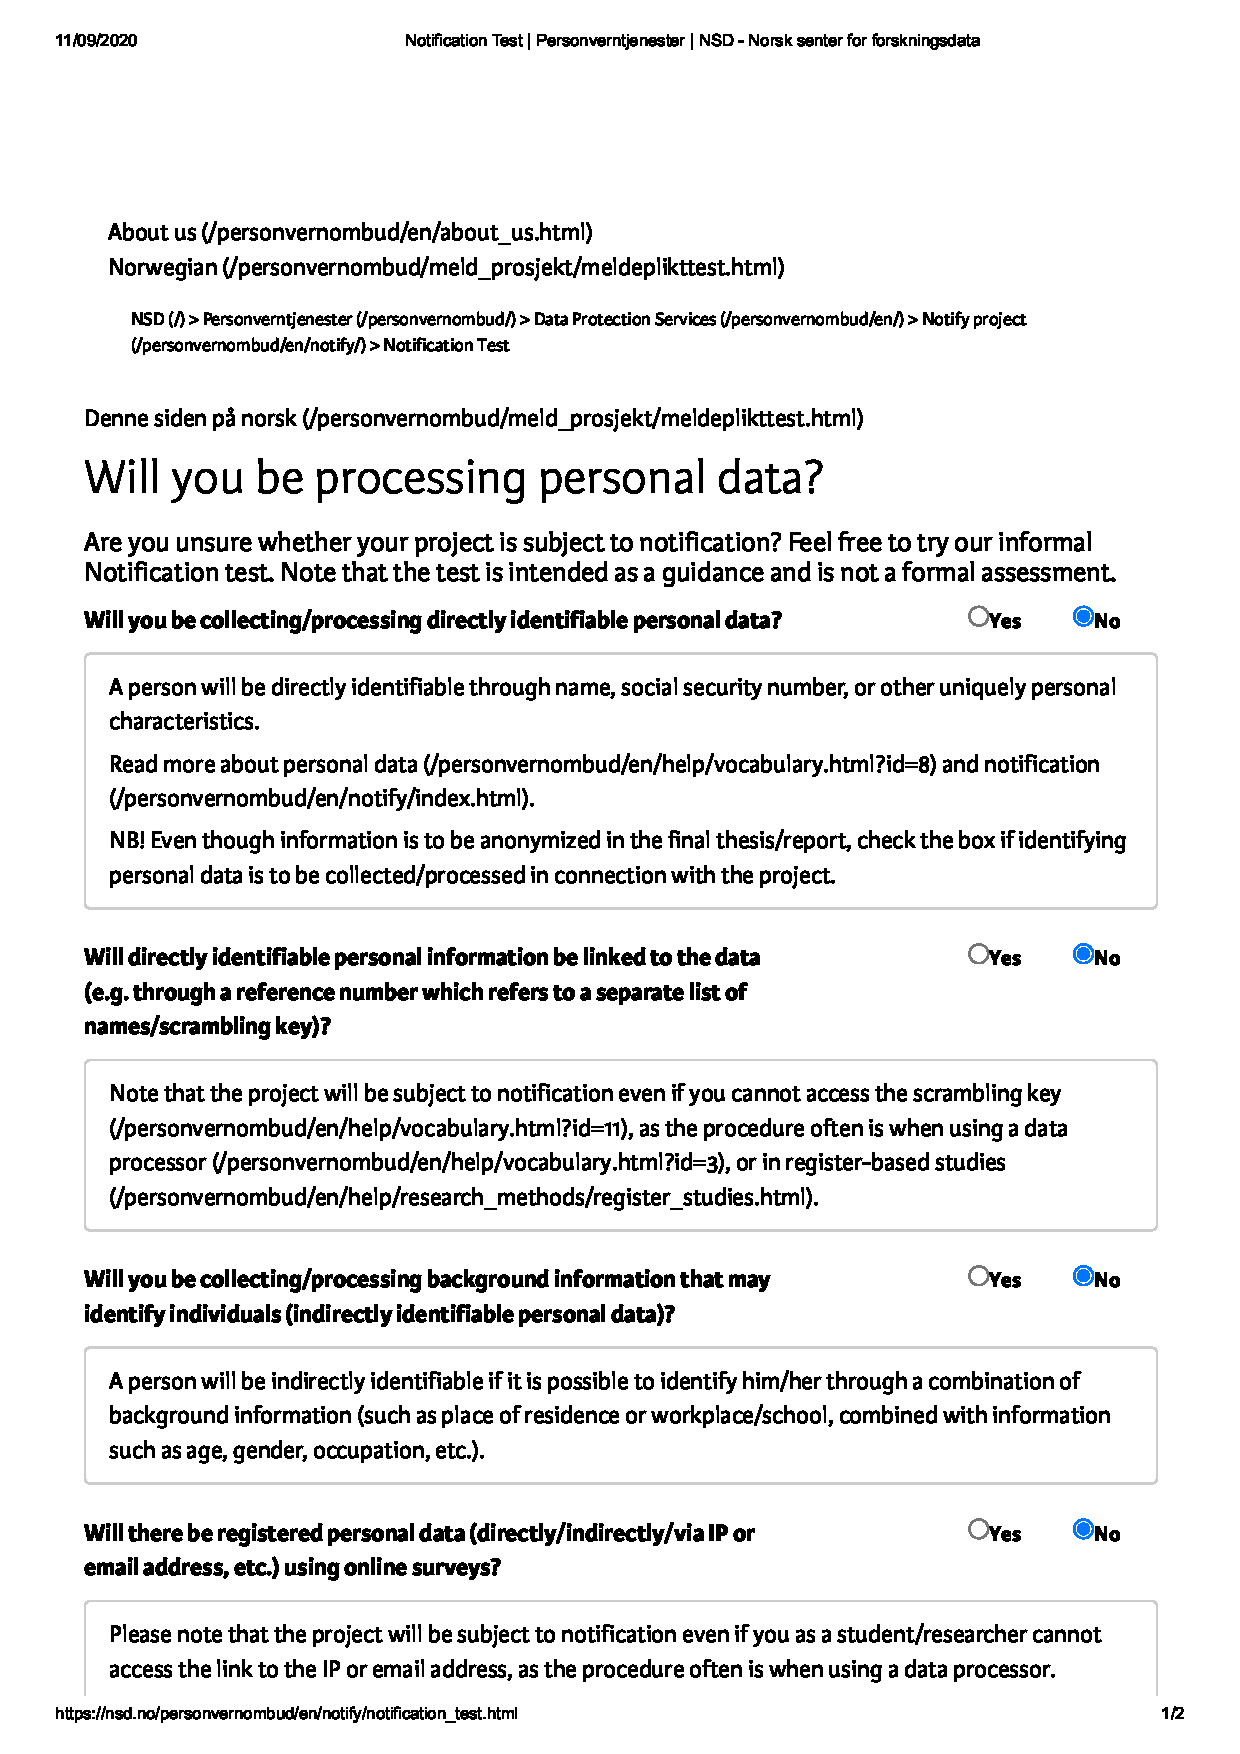
\includepdf[pages=-,fitpaper=true,noautoscale=true]{Appendices/Notification-Test.pdf}

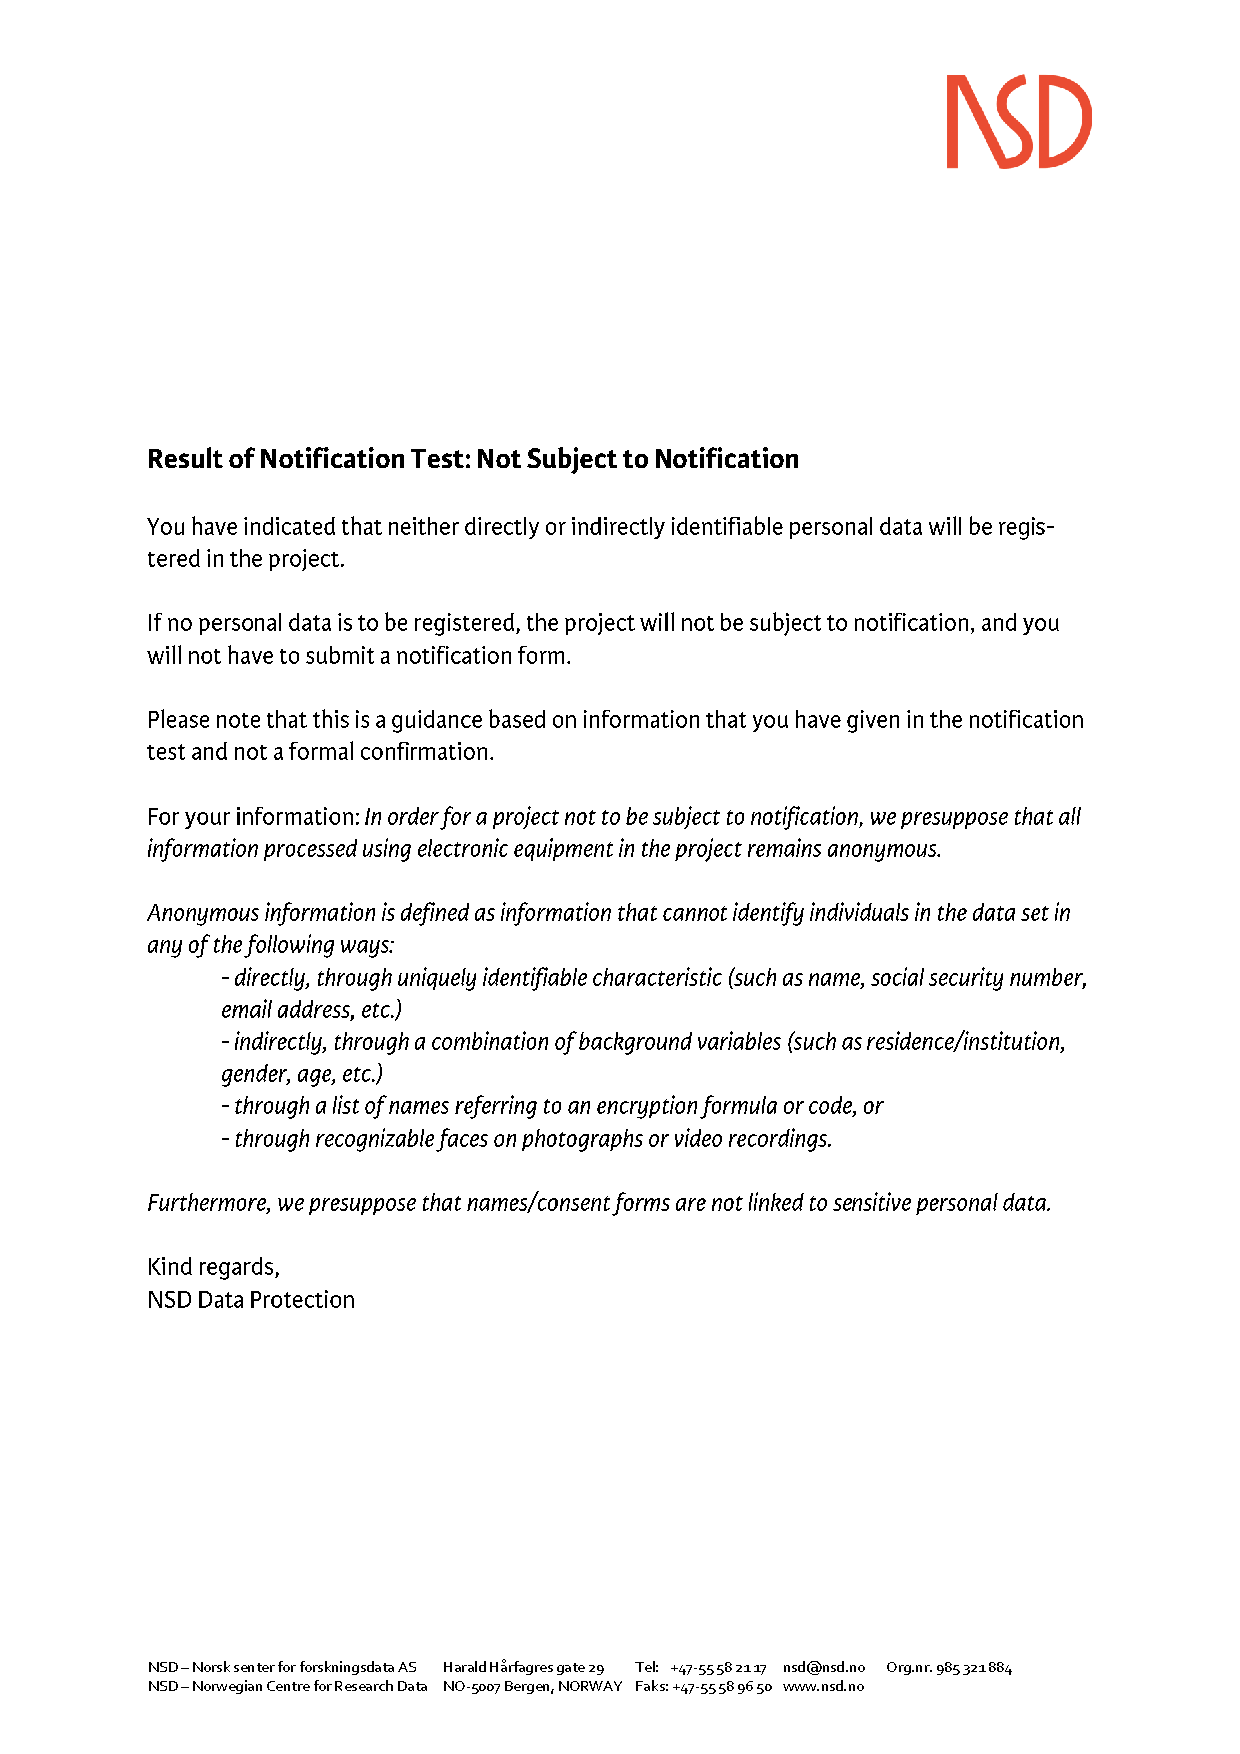
\includepdf[pages=-,fitpaper=true,noautoscale=true]{Appendices/not_subject_to_notification.pdf}


%    %\setcounter{secnumdepth}{0}
\chapter{Analysis Code}

\section{Chapter 1}

There is no analysis code in \cref{chp:1}.

\section{Chapter 2}

\subsection{Data Import} \label{R.import}
\begin{singlespace}\small
    \lstinputlisting[language=R,style=vscodeR]{./R/0 Import.R}
\end{singlespace}

\subsection{Missing Pattern Inspection} \label{R.missing}
\begin{singlespace}\small
    \lstinputlisting[language=R,style=vscodeR]{./R/1 Missing.R}
\end{singlespace}

\subsection{Data Reimport} \label{R.reimport}
\begin{singlespace}\small
    \lstinputlisting[language=R,style=vscodeR]{./R/2 Reimport.R}
\end{singlespace}

\subsection{Financial Knowledge Index} \label{R.fki}
\begin{singlespace}\small
    \lstinputlisting[language=R,style=vscodeR]{./R/4 FKI.R}
\end{singlespace}

%    \chapter{Derivation of Country-level Financial Knowledge Indices}

%\epigraph{There are two things you are better off not watching in the making: sausages and\\ econometric estimates.}{Edward Leamer}

\section{Theoretical Foundation}

PISA 2018 financial literacy dataset \parencite{FLdata} provides rich information about students and schools. For the purpose of cross-country comparison, however, the country-level data must be addressed separately by the researchers. \textcite{morenoherrero:2018a}, for instance, introduced a variable ``quality of math and science education'' to control for country-level differences since consensus is yet to emerge about the most appropriate measure for ``countries' financial knowledge''. Inspired by the UN's approach to forming Human Development Indices, a recent publication \textcite{olivermarquez:2020} highlighted four aspects of countries' macroeconomic practices in their attempt to develop country-level financial knowledge indices (FKI).

Oliver-M{\'a}rquez and colleagues consider a country's economic capability, represented by its GDP per capita, to be a key dimension in bringing about its FKI. Secondly, literature converges on the importance of education training for a country's financial knowledge capability \parencite{oecd:2005}. Thirdly, countries with regular engagement with sophisticated financial products and financial markets should possess higher FKI. Lastly, countries with higher aggregate consumption levels and with ageing populations are likely to possess higher FKI due to more frequent exposure and pressure in retirement provision, respetively.

More specifically, \textcite{olivermarquez:2020} suggests using the logarithm of GDP per capital in current international dollars (purchasing power parity adjusted) as a measure for the \texttt{Economic Capability} sub-index. For the \texttt{Education Training} sub-index, the authors consider postgraduate-to-total-tertiary-graduation ratios as a reflection of ``highly skilled'' workforce and the mean years of schooling as a measure of countries' general education levels. For the \texttt{Use} sub-index, gross portfolio equity assets (GPEA) and insurance company assets (ICA) are considered sophisticated financial products countries engage themselves in. Additionally, in order to capture the central role of technology in amplifying the proliferation and use of financial assets, the proportion of Internet users (\textsc{IUS}) enters the definition via
\[ \texttt{Use} = ( \text{GPEA} + \text{ICA} ) ^ \text{IUS}. \]
For the final sub-index \texttt{Need}, the authors define
\[ \texttt{Need} = ( \text{PFA} + \text{AC} ) ^ \text{AGEING}, \]
where \textsc{PFA} is the pension-fund-assets-to-\textsc{GDP} ratio. Aggregate consumption is defined as:
\[ \text{AC} = \frac{2\% \times \text{household final consumption expenditure}}{\text{GDP}}, \]
where the ``$2\%$ rule'' is drawn from \textcite{caliendo:2013} and the proportion of ageing population is computed as
\[ \text{AGEING} = \frac{ \left[ \frac{\text{population}(>65)}{\text{population}(20 \sim 64)} \right]_{2018} - \left[ \frac{\text{population}(>65)}{\text{population}(20 \sim 64)} \right]_{2009} }{ \left[ \frac{\text{population}(>65)}{\text{population}(20 \sim 64)} \right]_{2009} }. \]

\section{Data Collection and Missing Data Treatment}

The data sources for FKI computation are documented in \cref{tab:FKIsource} and its associated notes. The sub-indices \texttt{Educational Training} and \texttt{Use} both contain missing observations for the year 2018. Majority of such missing data appear to be the result of administrative delay, with historic observations available until 2017. It is therefore feasible to conduct time-series forecasts using prior year observations to best approximate 2018 values.

\ltable{tab:FKIsource}{Data Sources for FKI Computation}{
    \begin{tabular}{cclc}
    \toprule
    \multicolumn{1}{c}{Database$\ ^\text{a}$} & Country$\ ^\text{b}$ & \multicolumn{1}{c}{Series} & Time \\
    \midrule
    \rowcolor[rgb]{ .9,  .9,  .9} \multicolumn{4}{c}{Economic Capacity} \\
    WB-dev & 20    & GDP per capita, PPP (current international \$) & 2018 \\
    \rowcolor[rgb]{ .9,  .9,  .9} \multicolumn{4}{c}{Educational Training} \\
    WB-ed & 20 \textbackslash\ Russia & Graduates from ISCED 7 programmes in tertiary education, both sexes (number) & 2013--\textbf{2018} \\
          &       & Graduates from ISCED 8 programmes in tertiary education, both sexes (number) & 2013--\textbf{2018} \\
          &       & Graduates from tertiary education, both sexes (number) & 2013--\textbf{2018} \\
    RS & Russia & PhD (Type 1)$\ ^\text{c}$, PhD (Type 2)$\ ^\text{d}$ & 2018 \\
    RE & Russia & Master (Type 1)$\ ^\text{e}$, Master (Type 2)$\ ^\text{f}$, total tertiary \emph{excluding} PhD$\ ^\text{g}$ & 2018 \\
    HDR & 20    & Dimension = Education; Education = Mean years of schooling (years) & 2018 \\
    \rowcolor[rgb]{ .9,  .9,  .9} \multicolumn{4}{c}{Use} \\
    WB-fin & 20    & Gross portfolio equity assets to GDP (\%) & 2011--\textbf{2018} \\
           &       & Insurance company assets to GDP (\%) & 2011--\textbf{2018} \\
    WB-dev & 20    & Individuals using the Internet (\% of population) & 2009--\textbf{2018} \\
    \rowcolor[rgb]{ .9,  .9,  .9} \multicolumn{4}{c}{Need} \\
    WB-fin & 20 \textbackslash\ Georgia & Pension fund assets to GDP (\%) & 2008--\textbf{2018} \\
    GP & Georgia & Minutes of the meeting of the investment board of the Pension Agency$\ ^\text{h}$ & $\textcolor{white}{\ ^\text{*}}$2019$\ ^\text{*}$ \\
    GS & Georgia & GDP at current prices, billion GEL$\ ^\text{i}$ & 2018 \\
    WB-dev & 20    & Household and NPISHs final consumption expenditure, PPP (current international \$) & 2018 \\
          &       & GDP, PPP (current international \$) & 2018 \\
          &       & Population ages 0--14, male & 2009, 2018 \\
          &       & Population ages 0--14, female & 2009, 2018 \\
          &       & Population ages 15--64, male & 2009, 2018 \\
          &       & Population ages 15--64, female & 2009, 2018 \\
          &       & Population ages 65 and above, male & 2009, 2018 \\
          &       & Population ages 65 and above, female & 2009, 2018 \\
          &       & Population ages 15--19, male (\% of male population) & 2009, 2018 \\
          &       & Population ages 15--19, female (\% of female population) & 2009, 2018 \\
          \bottomrule
    \end{tabular}
}{Sub-indices are shaded in gray. Bold font signifies this year contains missing data.}{3}
\newpage

\begin{singlespace} \small
\begin{itemize}
    \item[$^\text{a}$] WB-dev = \href{https://databank.worldbank.org/source/world-development-indicators}{World Bank -- World development indicators}\\
        WB-ed = \href{https://databank.worldbank.org/source/education-statistics-^-all-indicators}{World Bank -- Education statistics -- All indicators}\\
        WB-fin = \href{https://databank.worldbank.org/source/global-financial-development}{World Bank -- Global financial development}\\
        HDR = \href{http://hdr.undp.org/en/data}{Human Development Reports -- Data}\\
        RS = \href{https://rosstat.gov.ru/}{Russian Federal State Statistic Service}\\
        RE = \href{https://minobrnauki.gov.ru}{Russian Ministry of Education and Science}\\
        GP = \href{https://www.pensions.ge}{Pension Agency of Georgia}\\
        GS = \href{https://www.geostat.ge}{National Statistics Office of Georgia}
    \item[$^\text{b}$] ``20'' = the 20 participating countries in 2018 \textsc{PISA} financial literacy test: Brazil, Bulgaria, Canada, Chile, Estonia, Finland, Georgia, Indonesia, Italy, Latvia, Lithuania, the Netherlands, Peru, Poland, Portugal, Russian Federation, Serbia, Slovak Republic, Spain, and the USA. ``\textbackslash'' = exluding or except
    \item[$^\text{c}$] \href{https://rosstat.gov.ru/storage/mediabank/asp-2(1).xls}{https://rosstat.gov.ru/storage/mediabank/asp-2(1).xls}, Sheet ``\foreignlanguage{russian}{по направлениям подготовки}'', Cell C7 = number of PhD graduates \mbox{(Type 1)}
    \item[$^\text{d}$] \href{https://rosstat.gov.ru/storage/mediabank/asp-3.xls}{https://rosstat.gov.ru/storage/mediabank/asp-3.xls}, Sheet ``\foreignlanguage{russian}{по научным специальностям}'', Cell B7 = number of PhD graduates \mbox{(Type 2)}
    \item[$^\text{e--g}$] \href{https://minobrnauki.gov.ru/common/upload/download/VPO_1_2018.rar}{https://minobrnauki.gov.ru/common/upload/download/VPO{\textunderscore}1{\textunderscore}2018.rar} contains a spreadsheet \textcolor{blue}{\foreignlanguage{russian}{СВОД{\textunderscore}ВПО1{\textunderscore}ВСЕГО}.xls}, Sheet ``P2{\textunderscore}1{\textunderscore}3(1)'', Cell E198 = number of master graduates (Type 1)$^\text{e}$, Cell E410 = number of master graduates (Type 2)$^\text{f}$, Cell E592 = total tertiary graduates \emph{excluding} PhD$^\text{g}$
    \item[$^\text{h}$] \href{https://www.pensions.ge/docs/legislation/investment-board-protocol-4.pdf}{Minutes of the meeting of the investment board of the Pension Agency}, p. 4, no. 3
    \item[$^\text{i}$] \href{https://www.geostat.ge/en/modules/categories/23/gross-domestic-product-gdp}{Gross domestic product (GDP)}, row = GDP at current prices, billion GEL, column = 2018
    \item[$^\text{*}$] Georgia started a \href{https://agenda.ge/en/news/2019/13}{new pension system} on 1 January 2019. Since 2018 was a transitional period with scarce data, 2019 is used as the best approximation for Georgia's pension system for 2018.
\end{itemize}
\end{singlespace}

\clearpage



\subsection{Sub-index \texttt{Educational Training}}

The 2018 archive for the number of master (ISCED 7), PhD (ISCED 8), and total tertiary graduates are incomplete for all participating countries except Georgia, Indonesia and Serbia. \cref{fig:skilled} presents a time series plot of
\[ \texttt{highly skilled} = \frac{\text{number of masters} + \text{number of PhDs}}{\text{total number of tertiary graduates}} \]
and suggests that this ratio is likely to be stable over time, especially between adjacent years. A ``naive forecast'', where the nearest available year's data are to be duplicated for 2018, is applied for \texttt{highly skilled}.

\pfigure{fig:skilled}{Proportion of Postgraduates to Total Tertiary Graduations}{1}{./Figures/skilled.pdf}{``Postgraduate'' is defined as master (ISCED 7) and PhD (ISCED 8) graduates. Countries not shown: GEO, IDN and SRB (2018 data available) and RUS (consult other sources)}{1.75}{1.25}

\subsection{Sub-index \texttt{Use}}

All series involved in calculating this sub-index, GPEA, ICA and IUS, contain missing data. When time series data contain only exponential growth but no underlying trend, a simple exponential smoothing would suffice \parencite{garder:1985}; if trend is present, Holt-Winters method is superior \parencite{chatfield:1978}. \cref{fig:use} facilitates this decision making by plotting both the original and log-transformed versions of GPEA and ICA series. Since curves after log-transformations have slopes, it is prudent to apply the Holt-Winters forecasting method in order to account for possible trends contained in the original series.

\pfigure{fig:use}{Time Series Trend Test}{1}{./Figures/use.pdf}{The time series plots after natural logarithm transformations (bottom panels) are not flat, suggesting the original series (top panels) contain trends. Holt-Winters method therefore is preferred over simple exponential smoothing for 2018 forecasts.}{0.5}{0.85}

The IUS series contains missing data for Canada, Chile and the United States. Similar Holt-Winters procedure is applied to recover 2018 IUS data.

\ltable{tab:FKIraw}{Data Utilised for Computing FKI}{
  \begin{tabular}{cd{3} c d{3}d{1} c d{3}d{3}d{3} c d{3}d{3}d{3}}
    \toprule
    & \multicolumn{1}{c}{Economic Capacity} &       & \multicolumn{2}{c}{Educational Training} &       & \multicolumn{3}{c}{Use} &       & \multicolumn{3}{c}{Need} \\
\cmidrule{2-2}\cmidrule{4-5}\cmidrule{7-9}\cmidrule{11-13}          & \multicolumn{1}{c}{GDP per capita} &       & \multicolumn{1}{c}{Skilled} & \multicolumn{1}{c}{Schooling} &       & \multicolumn{1}{c}{GPEA} & \multicolumn{1}{c}{ICA} & \multicolumn{1}{c}{IUS} &       & \multicolumn{1}{c}{PFA} & \multicolumn{1}{c}{AC} & \multicolumn{1}{c}{AGEING} \\
    \midrule
    BRA   & 9.612 &       & 6.484 & 7.8   &       & 1.683 & 16.259 & 70.434 &       & 11.827 & 1.21  & 0.288 \\
    BGR   & 10.026 &       & 45.294 & 11.8  &       & 4.114 & 7.044 & 64.782 &       & 13.577 & 1.091 & 0.234 \\
    CHL   & 10.117 &       & 16.371 & 10.4  &       & 51.755 & 25.591 & 89.531 &       & 73.225 & 1.073 & 0.214 \\
    EST   & 10.501 &       & 36.765 & 13    &       & 16.399 & 7.681 & 89.357 &       & 18.012 & 0.876 & 0.163 \\
    FIN   & 10.807 &       & 35.024 & 12.4  &       & 93.626 & 31.481 & 88.89 &       & 52.024 & 0.974 & 0.37 \\
    GEO   & 9.588 &       & 24.039 & 12.8  &       & 0.784 & 1.469 & 62.718 &       & 0.834 & 1.227 & 0.042 \\
    IDN   & 9.362 &       & 7.771 & 8     &       & 0.636 & 4.612 & 39.905 &       & 1.826 & 1.059 & 0.145 \\
    ITA   & 10.665 &       & 44.771 & 10.2  &       & 57.434 & 51.26 & 74.387 &       & 10.589 & 1.075 & 0.155 \\
    LVA   & 10.33 &       & 29.554 & 12.8  &       & 8.598 & 2.538 & 83.577 &       & 14.732 & 1.027 & 0.142 \\
    LTU   & 10.487 &       & 28.749 & 13    &       & 9.008 & 5.5   & 79.723 &       & 7.457 & 1.107 & 0.149 \\
    NLD   & 10.961 &       & 32.59 & 12.2  &       & 124.171 & 64.956 & 94.712 &       & 207.938 & 0.805 & 0.326 \\
    PER   & 9.479 &       & 13.577 & 9.2   &       & 16.027 & 6.505 & 52.54 &       & 22.53 & 1.187 & 0.227 \\
    POL   & 10.368 &       & 36.725 & 12.3  &       & 4.853 & 9.535 & 77.542 &       & 9.838 & 1.085 & 0.355 \\
    PRT   & 10.444 &       & 34.454 & 9.2   &       & 19.353 & 25.579 & 74.661 &       & 8.761 & 1.133 & 0.237 \\
    RUS   & 10.267 &       & 30.349 & 12    &       & 0.302 & 2.614 & 80.865 &       & 4.415 & 0.941 & 0.155 \\
    SRB   & 9.774 &       & 26.946 & 11.2  &       & 0.306 & 5.111 & 73.361 &       & 0.845 & 1.171 & 0.28 \\
    SVK   & 10.391 &       & 54.417 & 12.6  &       & 10.644 & 8.873 & 80.66 &       & 12.497 & 0.962 & 0.3 \\
    ESP   & 10.609 &       & 33.929 & 9.8   &       & 27.681 & 28.23 & 86.107 &       & 10.235 & 1.044 & 0.186 \\
    USA   & 11.048 &       & 24.825 & 13.4  &       & 55.505 & 30.183 & 84.881 &       & 150.04 & 1.364 & 0.252 \\
    \bottomrule
    \end{tabular}
}{Full variable names: Skilled = Postgraduate to total tertiary ratio; Schooling = Mean year of schooling; GPEA = Gross portfolio to GDP ratio; ICA = Insurance company assets to GDP ratio; IUS = Number of Internet users per 100 population; PFA = Pension fund assets to GDP ratio; AC = 2\% of household final consumption expenditure to GDP ratio; AGEING = Aged-to-productive-population ratio (\% change between 2009 and 2018)}{3}


\subsection{Other Items with Data Concerns}

Russia reported 67.96\% and 61.01\% of its total university degree receipients to be postgraduates for the year 2013 and 2015 respectively (2014 missing). This figure rapidly declines to 41.6\% in 2016 and further down to 25.69\% in 2017. Such volatility goes against the stable patterns shared by most countries in \cref{fig:skilled}, casting doubt on data reliability. Separate investigation is therefore conducted using Russian government archive (Notes c to g in \cref{tab:FKIsource}).

Georgia underwent pension reform in 2018 with fund balance gradually transitioning to State Pension Agency for its official resumption of duty on 1 January 2019. Resultantly, 2018 pension balance for this country is unavailable but to be best appoximated using 2019 official data (Notes h, i and * of \cref{tab:FKIsource}).

\cref{tab:FKIraw} documents the results of the abovementioned data recovery process.

\section{Standardisation, Weights and FKI}

Following \textcite{olivermarquez:2020}'s procedure, all series in \cref{tab:FKIraw} undergo min-max normalisation such that the smallest entry receives a new score of $0.01$ and the biggest number is re-coded to $0.99$. This slight deviation from the original paper (where the min-max normalisation yields $0$ to $1$) is to avoid multiplying a series by zero or raising a base to the power of zero.

Variable weights are calculated following \textcite{olivermarquez:2020}'s recipe to be the inverses of each series' standard deviations. Whereas a sub-index combines more than one series, each weight is further divided by the sum of the constituent weights so that total weights add to one.

FKI is finally computed by taking the geometric mean of all four sub-indices, subject to sub-index-weights similar to variable weights above, as presented in \cref{tab:FKI}.

\ptable{tab:FKI}{FKI and Sub-indices}{
    \begin{tabular}{c c d{3} c d{3}d{3}d{3}d{3}}
\toprule
        && \multicolumn{1}{c}{FKI}       && \multicolumn{1}{c}{EC}        & \multicolumn{1}{c}{ET}        & \multicolumn{1}{c}{Use}       & \multicolumn{1}{c}{Need}\\
\midrule
        USA   &       & 1.029 &       & 0.990 & 0.590 & 1.467 & 1.580 \\
        ITA   &       & 0.810 &       & 0.767 & 0.601 & 1.603 & 0.767 \\
        ESP   &       & 0.661 &       & 0.734 & 0.464 & 1.012 & 0.670 \\
        LTU   &       & 0.609 &       & 0.664 & 0.633 & 0.325 & 0.801 \\
        PRT   &       & 0.606 &       & 0.639 & 0.401 & 0.869 & 0.719 \\
        CHL   &       & 0.589 &       & 0.449 & 0.302 & 1.372 & 0.939 \\
        EST   &       & 0.576 &       & 0.672 & 0.747 & 0.419 & 0.455 \\
        SVK   &       & 0.552 &       & 0.608 & 0.924 & 0.414 & 0.341 \\
        POL   &       & 0.546 &       & 0.595 & 0.700 & 0.354 & 0.503 \\
        GEO   &       & 0.369 &       & 0.141 & 0.548 & 0.174 & 0.997 \\
        PER   &       & 0.289 &       & 0.078 & 0.194 & 0.780 & 0.868 \\
        BRA   &       & 0.131 &       & 0.155 & 0.010 & 0.506 & 0.809 \\
        IDN   &       & 0.104 &       & 0.010 & 0.040 & 0.975 & 0.734 \\
\bottomrule
    \end{tabular}
}{Table sorted in descending order by countries' FKI. FKI = financial knowledge index, EC = Economic Capability, ET = Educational Training.}{2.5}


%    \chapter{Multilevel Multiple Imputation}
\label{app:MMI}

\section{\textsf{Mplus} Input Code}
\label{sec:MMI_inp}

\lstinputlisting[style=vscodeMplus]{./Mplus/MMI/MMI.inp}

\section{Selected \textsf{Mplus} Output}
\label{sec:MMI_out}

\lstinputlisting[style=vscodeMplus_out,linerange={2909-2967}]{./Mplus/MMI/MMI.out}

\section{Diagnostic Plots}
\label{sec:MMI_diagnostic}

\newpage

% Table generated by Excel2LaTeX from sheet 'Sheet1'
\ltable{tab:MMI}{Summary of Diagnostic Plots of Multilevel Multiple Imputation}{
      \begin{tabular}{ccclrrccc}
\toprule
      Parameter & \multicolumn{1}{c}{Parameter} & Modelling & \multicolumn{1}{c}{Brief} & \multicolumn{1}{c}{Posterior} & \multicolumn{1}{c}{Posterior} & 95\% credibility & Chain & AR-free \\
      number & \multicolumn{1}{c}{label} & level & \multicolumn{1}{c}{description} & \multicolumn{1}{c}{mean} & \multicolumn{1}{c}{variance} & interval & converged & chains \\
\midrule
      1     & \texttt{MALE}  & Within & Whether participant is male & 0.502 &       & (0.499, 0.505) & Yes   & 4 \\
      2     & \texttt{IMMI1GEN} & Within & Whether participant migrated to this country & 0.029 &       & (0.028, 0.030) & Yes   & 4 \\
      3     & \texttt{IMMI2GEN} & Within & Whether their parent did & 0.042 &       & (0.041, 0.044) & Yes   & 4 \\
      4     & \texttt{ESCS}  & Within & Index of economic, social and cultural status & $-$0.241 &       & ($-$0.247, $-$0.234) & Yes   & 4 \\
      5     & \texttt{FCFMLRTY} & Within & Familiarity with concepts of finance & 7.049 &       & (7.015, 7.083) & Yes   & 4 \\
      6     & \texttt{FLCONFIN} & Within & Confidence about financial matters & $-$0.072 &       & ($-$0.079, $-$0.065) & Yes   & 4 \\
      7     & \texttt{FLSCHOOL} & Within & Financial education in school lessons & 0.018 &       & (0.011, 0.024) & Yes   & 4 \\
      8     & \texttt{NOBULLY} & Within & Participant's experience of being bullied (reverse) & $-$0.059 &       & ($-$0.067, $-$0.052) & Yes   & 4 \\
      9     & \texttt{FLFAMILY} & Within & Parental involvement in matters of financial literacy & 0.064 &       & (0.057, 0.070) & Yes   & 4 \\
            &       &       &       &       &       &       &       &  \\
      10    & \texttt{MALE}  & Within & Whether participant is male &       & 0.250 & (0.248, 0.252) & Yes   & 4 \\
      11    & \texttt{IMMI1GEN} & Within & Whether participant migrated to this country &       & 0.028 & (0.028, 0.028) & Yes   & 4 \\
      12    & \texttt{IMMI2GEN} & Within & Whether their parent &       & 0.041 & (0.040, 0.041) & Yes   & 4 \\
      13    & \texttt{ESCS}  & Within & Index of economic, social and cultural status &       & 1.183 & (1.173, 1.193) & Yes   & 4 \\
      14    & \texttt{FCFMLRTY} & Within & Familiarity with concepts of finance &       & 29.754 & (29.495, 30.016) & Yes   & 4 \\
      15    & \texttt{FLCONFIN} & Within & Confidence about financial matters &       & 1.034 & (1.025, 1.044) & Yes   & 4 \\
      16    & \texttt{FLSCHOOL} & Within & Financial education in school lessons &       & 1.040 & (1.031, 1.049) & Yes   & 4 \\
      17    & \texttt{NOBULLY} & Within & Participant's experience of being bullied (reverse) &       & 1.111 & (1.100, 1.121) & Yes   & 4 \\
      18    & \texttt{FLFAMILY} & Within & Parental involvement in matters of financial literacy &       & 1.090 & (1.080, 1.100) & Yes   & 4 \\
            &       &       &       &       &       &       &       &  \\
      19    & \texttt{STRAIO} & Between & Student$-$teacher ratio & 13.873 &       & (13.607, 14.139) & Yes   & 4 \\
      20    & \texttt{EDUSHORT} & Between & Shortage of educational material & 0.131 &       & (0.106, 0.157) & Yes   & 4 \\
            &       &       &       &       &       &       &       &  \\
      21    & \texttt{STRAIO} & Between & Student$-$teacher ratio &       & 103.532 & (99.750, 107.430) & Yes   & 4 \\
      22    & \texttt{EDUSHORT} & Between & Shortage of educational material &       & 1.074 & (1.037, 1.112) & Yes   & 4 \\
\bottomrule
      \end{tabular}
}{Notes go here.}{6}
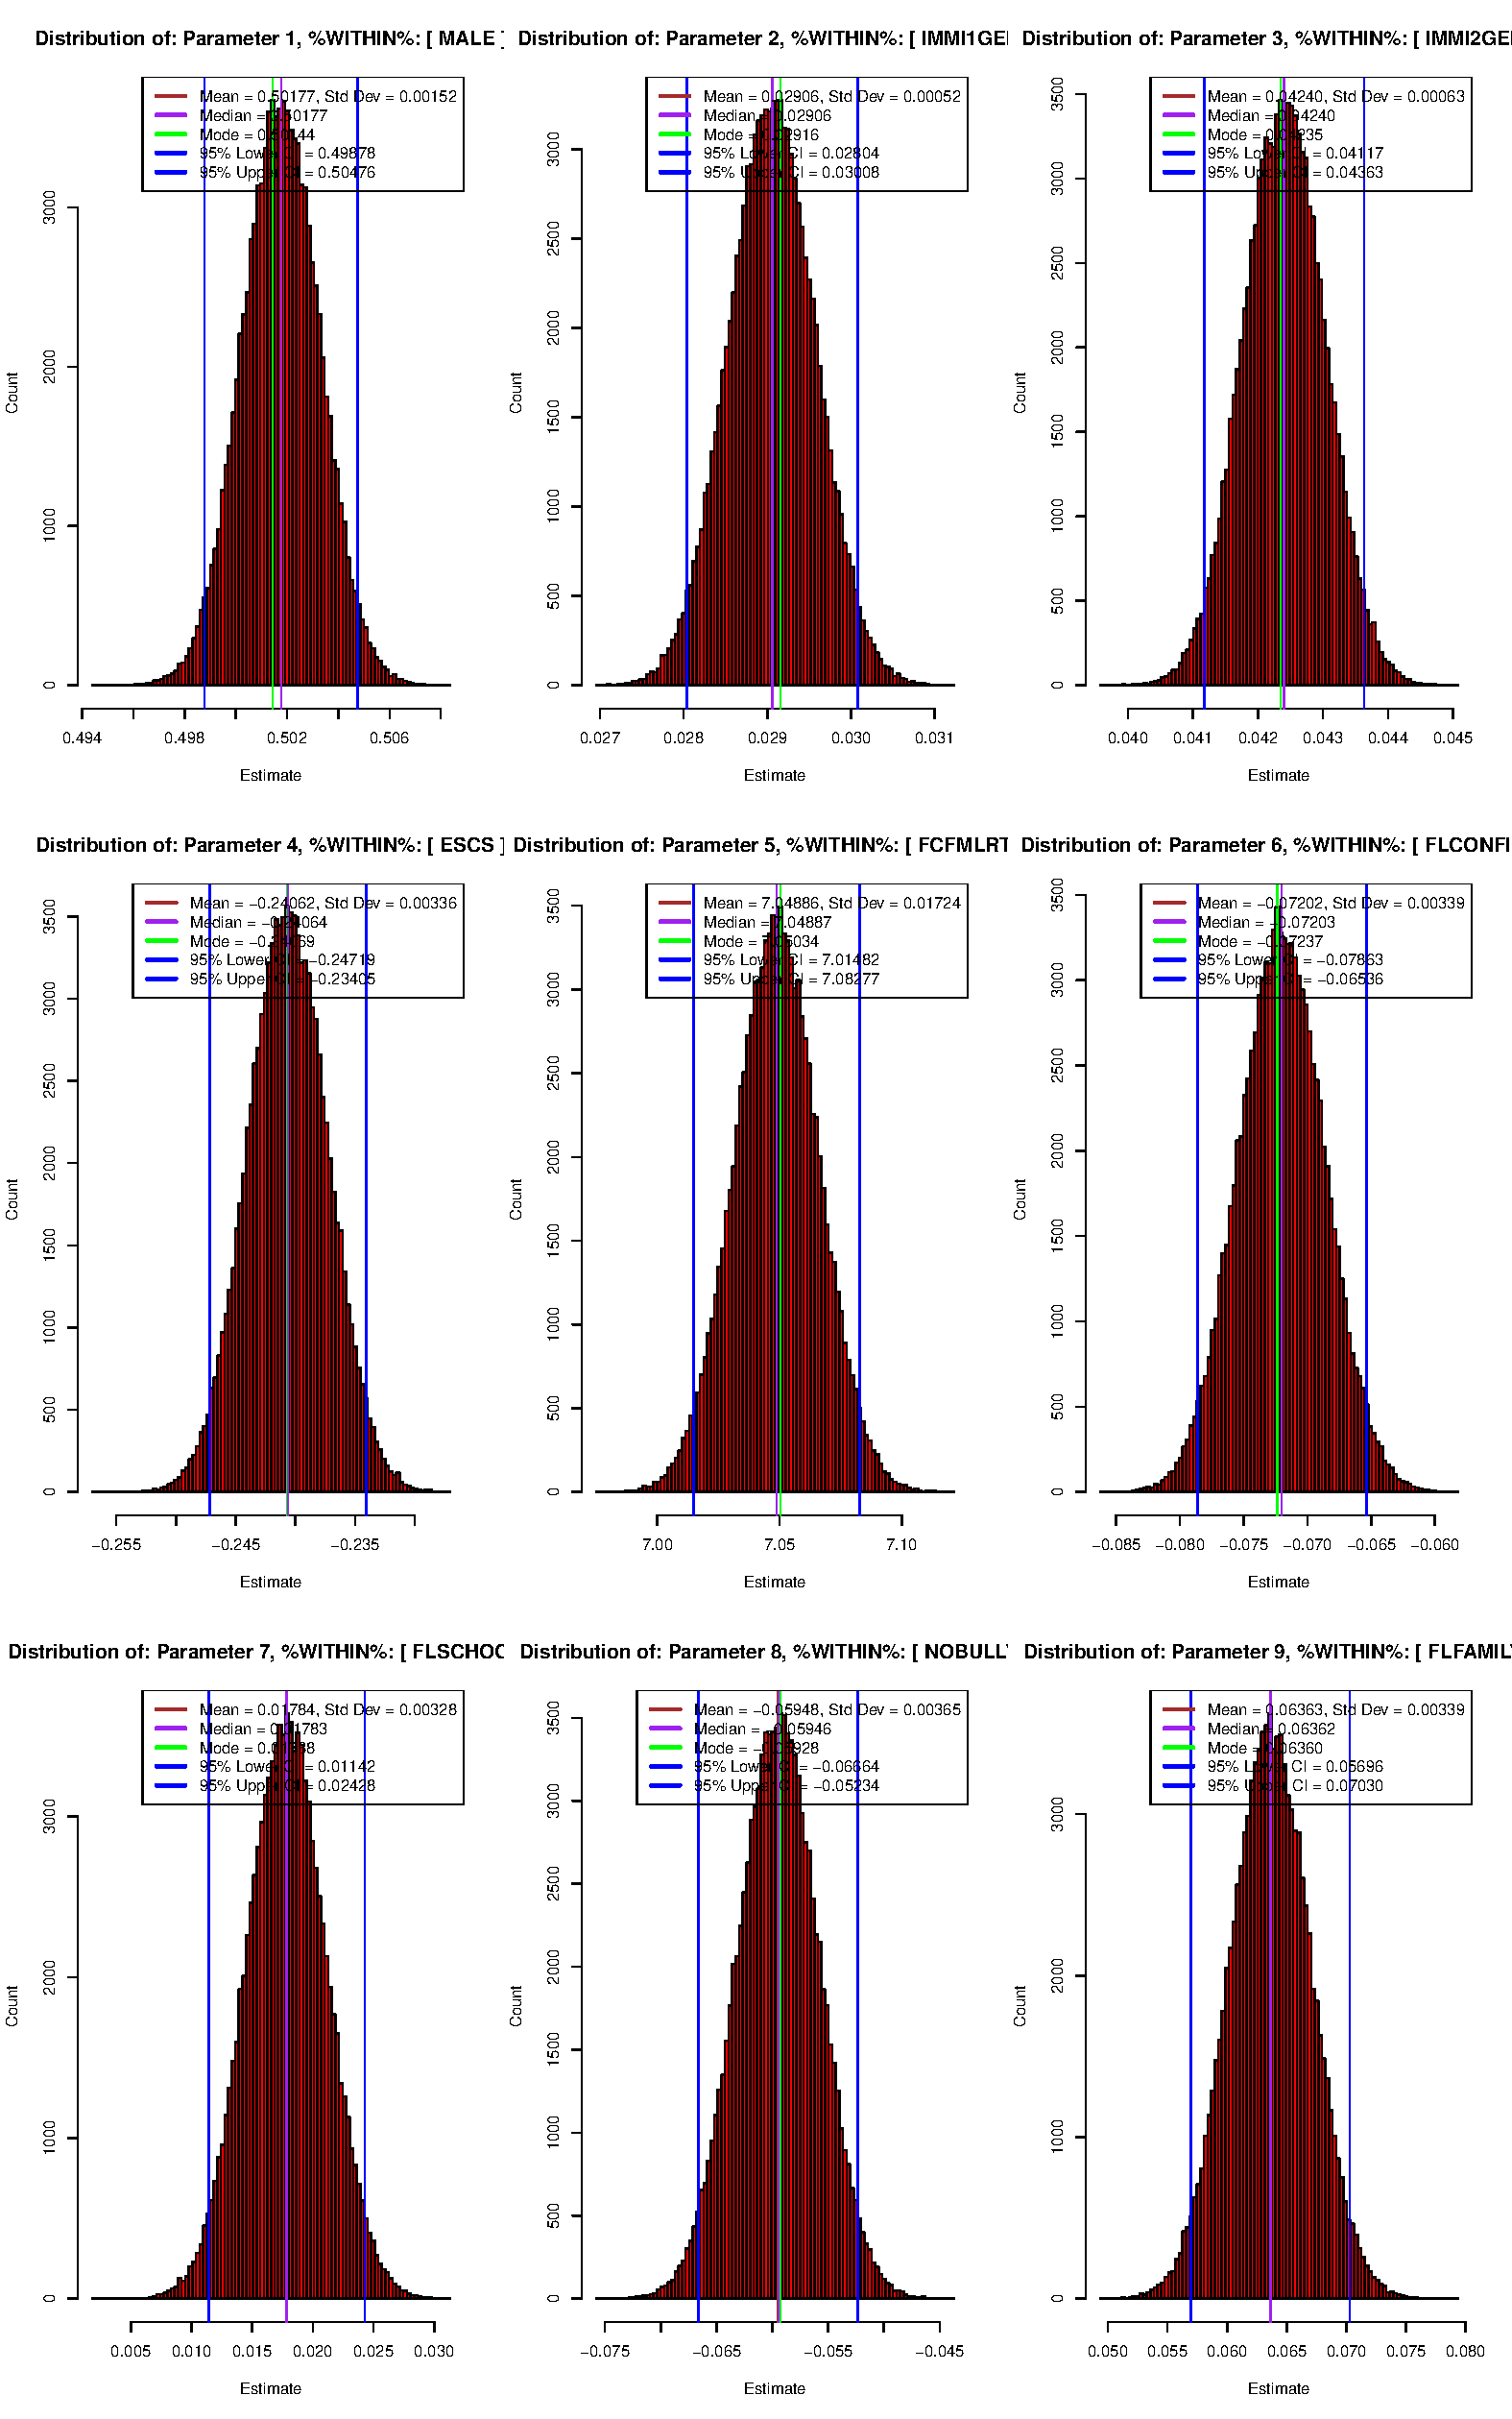
\includepdf[pages=-,width=\textwidth]{./Figures/MMI_diagnostic.pdf}

%    \include{Appendices/E}
%    \include{Appendices/F}
\end{appendices}

% Put Index here
%\begin{multicols}{2}
\cleardoublepage
\phantomsection
\addcontentsline{toc}{chapter}{Name Index}
\printindex[a]

\cleardoublepage
\phantomsection
\addcontentsline{toc}{chapter}{Subject Index}
\printindex
%\end{multicols}

\end{document}
